%%%%%%%%%%%%%%%%%%%%%%% file template.tex %%%%%%%%%%%%%%%%%%%%%%%%%
%
% This is a general template file for the LaTeX package SVJour3
% for Springer journals.          Springer Heidelberg 2010/09/16
%
% Copy it to a new file with a new name and use it as the basis
% for your article. Delete % signs as needed.
%
% This template includes a few options for different layouts and
% content for various journals. Please consult a previous issue of
% your journal as needed.
%
%%%%%%%%%%%%%%%%%%%%%%%%%%%%%%%%%%%%%%%%%%%%%%%%%%%%%%%%%%%%%%%%%%%
%
% First comes an example EPS file -- just ignore it and
% proceed on the \documentclass line
% your LaTeX will extract the file if required
\begin{filecontents*}{example.eps}
%!PS-Adobe-3.0 EPSF-3.0
%%BoundingBox: 19 19 221 221
%%CreationDate: Mon Sep 29 1997
%%Creator: programmed by hand (JK)
%%EndComments
gsave
newpath
  20 20 moveto
  20 220 lineto
  220 220 lineto
  220 20 lineto
closepath
2 setlinewidth
gsave
  .4 setgray fill
grestore
stroke
grestore
\end{filecontents*}
%
\RequirePackage{fix-cm}
%
%\documentclass{svjour3}                     % onecolumn (standard format)
\documentclass[smallcondensed]{svjour3}     % onecolumn (ditto)
%\documentclass[smallextended]{svjour3}       % onecolumn (second format)
%\documentclass[twocolumn]{svjour3}          % twocolumn
%
\smartqed  % flush right qed marks, e.g. at end of proof
%
\usepackage{graphicx}
%
\usepackage{mathptmx}      % use Times fonts if available on your TeX system
%
% insert here the call for the packages your document requires
%\usepackage{latexsym}
\usepackage{adjustbox}
\usepackage{amssymb}
%\usepackage{amsthm}
\usepackage{newtxmath}
\usepackage{amsmath}  
%\usepackage{natbib}
% etc.
%
% please place your own definitions here and don't use \def but
% \newcommand{}{}
%
% Insert the name of "your journal" with
\journalname{Quality \& Quantity - International Journal of Methodology}
%
\begin{document}

\title{A Network Agent-Based Model of Ethnocentrism and Intergroup Cooperation\thanks{Funding for this research was provided by the Research Council of Norway (grant \#250449).}
}
%\subtitle{Do you have a subtitle?\\ If so, write it here}

%\titlerunning{Short form of title}        % if too long for running head

\author{Carlos M. Lemos \and
	Ross J. Gore \and
	Laurence Lessard-Phillips \and 
	F. LeRon Shults%etc.
}

%\authorrunning{Short form of author list} % if too long for running head

\institute{Carlos M. Lemos  \at
	 Department of Religion, Philosophy and History, University of Agder, Norway \\
	\email{carlos.lemos@uia.no}           %  \\
	%             \emph{Present address:} of F. Author  %  if needed
	\and
	Ross J. Gore \at
	Virginia Modeling, Analysis and Simulation Center, Old Dominion University, Norfolk, VA, United States of America \and
	Laurence Lessard-Phillips \at 
	Institute for Research into Superdiversity (IRiS), School of Social Policy, University of Birmingham, Birmingham, United Kingdom \and
	F. LeRon Shults \at
	Institute for Global Development and Social Planning, University of Agder, Norway\\
	Center for Modeling Social Systems at NORCE, Kristiansand, Norway	
}

\date{Received: date / Accepted: date}
% The correct dates will be entered by the editor


\maketitle

\begin{abstract}
We present a network agent-based model of ethnocentrism and intergroup cooperation in which agents from two groups  (majority and minority) change their communality (feeling of group solidarity), cooperation strategy and social ties, depending on a barrier of ``likeness'' (affinity). Our purpose was to study the model's capability for describing how the mechanisms of preexisting markers (or ``tags'') that can work as cues for inducing in-group bias, imitation, and reaction to non-cooperating agents, lead to ethnocentrism or intergroup cooperation and influence the formation of the network of mixed ties between agents of different groups. We explored the model's behavior via four experiments in which we studied the combined effects of ``likeness,'' relative size of the minority group, degree of connectivity of the social network, game difficulty (strength) and relative frequencies of strategy revision and structural adaptation. The parameters that have a stronger influence on the emerging dominant strategies and the formation of mixed ties in the social network are the group-tag barrier, the frequency with which agents react to adverse partners, and the game difficulty. The relative size of the minority group also plays a role in increasing the percentage of mixed ties in the social network. This is consistent with the intergroup ties being dependent on the ``arena'' of contact (with progressively stronger barriers from e.g. workmates to close relatives), and with measures that hinder intergroup contact also hindering mutual cooperation.


\keywords{Ethnocentrism \and Agent-based model \and Cooperation in Networks}
% \PACS{PACS code1 \and PACS code2 \and more}
% \subclass{MSC code1 \and MSC code2 \and more}
\end{abstract}

\section{Introduction}
\label{intro}
Ethnocentrism can be defined as the tendency for behaving differently towards people belonging to the same group (in-group) than towards people belonging to some other group (out-group) (Levine and Campbell 1972). It can also be considered as a form of in-group bias, or as a tendency for cooperating with in-group members but not with out-group members (Brewer 1999). Studies of ethnocentrism and ethnocentric behavior are often linked to the changing ethno-national landscape in many societies. Ethnocentrism is an ubiquitous behavioral pattern in societies, which although not necessarily implying hostility towards out-groups (xenophobia) is related to social phenomena ranging from voting behavior (Kinder 1998), to segregation and discrimination towards minority groups (Perreault and Bourhis 1999), and even ethnic conflict (Brewer 1979; Chirot and Seligman 2001) and war (van der Dennen 1995). There is strong empirical evidence for the prevalence of in-group bias in several contexts (Brewer 1979; Kramer and Breuer 1984; Yamagishi and Mifune 2009). It is also well known that this can be triggered even by minimal cues that set arbitrary group boundaries (Tajfel et al. 1971; Doise et al. 1972; Ahmed 2007), and that inequality hinders intergroup interactions while heterogeneity promotes them (Blau 1997). 


Due to its importance within social sciences, ethnocentrism has been studied from the viewpoints of sociology (Blau 1977; McPherson et al. 2001), social psychology, cognitive science, and also game theory (Axelrod 1984; Macy and Flache 2002; Dixit et al. 2015), evolutionary dynamics and evolutionary biology (Smith 1882; Nowak 2006; Nowak 2006a). More recently, ethnocentrism and related phenomena have been studied by means of modeling and simulation, using agent-based models (ABMs). Several ABMs have been proposed for describing outcomes of the interaction between populations of individuals with different characteristics, such as spatial segregation (Schelling 1971), local uniformity and global polarization of cultural traits (Axelrod 1997), ethnocentrism (Hammond and Axelrod 2006), and the link between individual strategies and the structural properties of social networks in which cooperation evolves (e.g. Santos et al. 2006; Santos et al. 2006a; Pinheiro et al. 2012; Santos et al. 2016). 

In this paper we build on the models above and present a network ABM of ``abstract'' type for describing the co-evolution of ethnocentrism and social ties between two groups of unequal size. The model's purpose is to describe how the patterns of in- and out-group cooperation and the structure of the network of mixed ties are influenced by relative group size, cooperation barriers and frequency of adaptation to adverse ties (non-cooperating link neighbors). The research questions we wanted to answer are:
\begin{enumerate}
	\item How do the barriers of game difficulty and group tag influence the emergent strategies of the two groups?
	\item What is the influence of structural adaptation on the emergence of full cooperation between the two groups?
	\item What is the influence of relative size of the minority group and initial average connectivity on the emerging dominant strategies of each group and the formation of the network of mixed ties?
\end{enumerate}

The innovation of the present model with respect to previous ABMs related to acculturation and ethnocentrism is the combination of (\emph{i}) network (instead of spatial) interactions; (\emph{ii}) a tag-induced social barrier; and (\emph{iii}) a parsimonious model for the co-evolution of strategy and structure within the network. This allowed us to show that the group-tag barriers play a key role in determining which strategies will emerge as dominant, and that our model is capable of generating diversity, in the sense that strategies other than dominant persist within both minority and majority groups. Also, the agents' ability to react to non-cooperating partners promotes ethnocentric and full cooperation.

The remainder of this paper is organized as follows. In section two, we present an overview of ABMs that have been proposed for describing the emergence of ethnocentric behavior between groups and cooperation in networks that we use in our model. Section three contains a description of the model. In section four we present the results of computer experiments that show the model's capability for representing different outcomes of emergent strategies and mixed ties between the two groups. Sections five and six contain a discussion of the results and some notes about the model's limitations, respectively. Finally, section seven contains a summary of conclusions and prospects for future work.

\section{Theoretical Background}
Many ABMs have been proposed to describe social phenomena related to ethnocentrism and cooperation in spatial environments or networks. All these models are of the ``abstract'' type (Gilbert 2007), as their purpose is to describe the key mechanisms that explain emergent (macroscopic) patterns in terms of a small number of agent types, endowed with simple interaction rules and behaviors. For example, Schelling's model of spatial segregation (Schelling 1971; Schelling 2006) and Axelrod's ABM of dissemination of culture (Axelrod 1997), describe spatial segregation due to homophily, and local uniformity/global polarization of cultural traits, respectively. However, these ABMs will not be further explored here, as they are not directly relevant to our model.

Hammond and Axelrod (2006) proposed an ABM for describing the emergence of ethnocentric behavior. In this model agents are of a single type and have three traits: a color/ethnicity tag (with two possible values), cooperation/defection towards agents of the in-group and cooperation/defection towards agents of the out-group. Hammond and Axelrod's model is based on a combination of ideas from population dynamics (by including immigration and death), and the PD framework (without iteration) for the agents' interactions, and evolutionary models (agents die before transmitting their strategy traits to offspring if their potential to reproduce (PTR) is insufficient; and strategies suffer mutations in the reproduction process). The main finding of Hammond and Axelrod is that according to their ABM ethnocentric behavior strongly prevails under a wide range of conditions.

Hammond and Axelrod's model has been criticized in several other aspects. For example, this model does not take into account the mechanisms of reciprocity and transitivity (Nowak 2006). Also, because offspring agents are created in their parents' neighborhood, the emergent patterns result from kin selection instead of ethnocentrism (Jansson 2015).

One feature of most of the aforementioned models is that interactions between agents occur in neighborhoods of a spatial grid. This not only restricts the resulting emergent patterns but also fails to represent many real life problems in which relevant interactions occur in networks (Epstein 2006). The literature on decision, strategic games and cooperation in networks is vast (see e.g. Jackson (2008), Ohtsuki et al. (2006) or Santos et al. (2006a)), so we will only describe in greater detail the approach we found most useful for developing our model.

It is well known that models of cooperation in networks must combine strategy and structural changes (Skyrms and Pemantle 2000). The challenge has been to represent these mechanisms in a simple and parsimonious way. Santos, Pacheco and Lenaerts (2006) proposed a model of cooperation in networks (hereafter called SPL) in which agents both change behavior and adjust their ties. In this model, agents are of a single type and play a social dilemma game with their link neighbors. They update their behavior (cooperate or defect) by imitating the strategy of link neighbors with a probability given by a logistic function of the difference between their respective payoffs. Agents also try to get rid of adverse ties (link neighbors that do not cooperate) by rewiring from defecting agents to link neighbors of the latter, with a probability that is also a logistic function of their respective payoffs. In this model no agents are created or die (no population dynamics). Also, rewiring can only occur if the network remains connected and strategy and structural updates are not simultaneous.

In the SPL model, the relative time scale of behavior and structural updates is controlled by a parameter $ \tau $ such that $ \tau = 0 $ leads to no structural updates (static networks) and $ \tau = 1 $ to no behavioral updates. The details of this model, as well as developments and applications can be found in e.g. Santos et al. (2006), Pinheiro et al. (2012), Santos et al. (2016) and Pinheiro et al. (2016). Santos et al. (2006) considered three social dilemmas of cooperation: the ``Chicken run'' (or ``Snow drift'') game, in which players are greedy and prefer defection to mutual cooperation; the ``Stag Hunt'' game, in which cooperation entails a risk; and the PD game, which combines both greed and risk. The key results obtained with this model were that structural adaptation favors the emergence of cooperation and that there is a critical value for  $ \tau $ beyond which cooperators wipe out defectors (Santos et al. 2006). This model is important for the present work because of its simplicity and generative power. Nevertheless, it does not describe strategy and structural updates arising from two groups (majority and minority) when some tag-induced barrier to cooperation exists. Therefore, it cannot represent how different combinations of in- and out-group strategies and the network of mixed ties emerge in a mixed artificial society. Our model attempts to improve these issues.

\section{Model Description}
In this section we describe our proposed ABM. The model was implemented in NetLogo (Wilensky 1999). Experiments involving multiple sweeping parameters and outputs (e.g. global dependent variables, agent attributes, and networks) were run via a R-script using the \texttt{RNetLogo} (Thiele et al. 2012; Thiele 2014) and \texttt{doParallel} packages within \texttt{R} (R Core Team 2016).

\subsection{Purpose, Entities and Scales}
The model's purpose is to describe the co-evolution of in- and out-group cooperation and inter-group ties for two groups connected in a social network, under the influence of tag-induced barriers to cooperation.

The model entities are the agents and a social network that connects them. Agents belong to two groups, defined by a group tag with values ``blue'' and ``green'' for majority and minority groups, respectively. They have an attribute called ``communality,'' which in abstract stands for ``feeling of group solidarity, '' and that we model as the payoff of a social dilemma game as described next. At each time step, they can change their communality by trying to play a social dilemma game with their link neighbors. The probability of a successful pairwise interaction (leading to one-shot game play) is conditioned by their individual ``likenesses'' (or ``affinities'') towards each other, which depends on the groups to which the interacting agents belong. This setting of the micro-interactions is consistent with Blau's theory of intergroup contact (Blau 1977) and the McPherson et al. (2001) theory on the importance of homophily in shaping social networks (McPherson 2001). Agents then try to improve their communality by either revising their strategies or by getting rid of non-cooperative partners. 
\begin{table}[t!] \centering
	\small
	\begin{tabular}{lll}
		%\begin{tabularx}{\textwidth}{XXXX}
		\hline
		\textbf{Process} & \textbf{Mechanism}  & \textbf{Theoretical Foundation}  \\
		\hline
		\rule{0pt}{0ex} Interaction barrier & in-group bias & General empirical evidence \\
		& & (Tajfel et al. 1971; Levine and Campbell 1972; Brewer 1979)\\
		\rule{0pt}{4ex} Cooperation barrier  & greed and/or fear & Game theory, social dilemma games \\
		& & (Macy and Flache 2002; Nowak 2006)\\
		\rule{0pt}{4ex} Strategy change    & imitation & Games in networks \\
		& & (Skyrms and Pemantle 2000; Ebel 2002; Santos et al. 2006)\\
		\rule{0pt}{4ex} Structural change & adaptation & Games in networks \\
		& & (Skyrms and Pemantle 2000; Ebel 2002; Santos et al. 2006)\\		
		\hline
	\end{tabular}
	%\end{tabularx}
	\caption{Main processes, mechanisms and theoretical foundations considered in the model}
	\label{tab:Processes}
\end{table}

Table \ref{tab:Processes} summarizes the mechanisms and processes considered in the model. There is general empirical evidence that an in-group bias exists in many contexts (Tajfel et al. 1971; Levine and Campbell 1972; Brewer 1979). Introduction of a tag-induced barrier for conditioning the success (or effectiveness) of individual interactions is a simple form of representing this bias. Barriers to cooperation and strategy changes are basic mechanisms in the context of social dilemma games (Rapoport 1999; Nowak 2006a; Dixit et al. 2015). Finally, the coupling of strategy and structural changes is a key mechanism for modeling the emergence of cooperation in networks (Skyrms and Pemantle 2000; Ebel 2002; Santos et al. 2006).

Tables \ref{tab:GlobalVariables} and \ref{tab:AgentAttributes} show the global variables and the agents' attributes, respectively. The meaning of the variables and attributes will be explained below, as they are progressively introduced. The total number of agents is determined by the \texttt{numAgents} global variable. The number of agents of each group is set by fixing the proportion of ``green'' agents (\texttt{propGreen}). In this work, the ``green'' population will be the minority group. The social network is initialized using the small-world model (Watts and Strogatz 1998), with initial average node degree (initial average number of link neighbors of the agents)  and rewiring probability defined by the $ n_W $ and $ p_{rewire} $ global variables, respectively. In this way the artificial society (including both populations) is initially connected so that the clustering coefficient is high and the ``social distance'' is controlled by $ p_{rewire} $. 
\begin{table}[t!] \centering
	\small
	\begin{tabular}{llll}
		%\begin{tabularx}{\textwidth}{XXXX}
		\hline
		\textbf{Variable} & \textbf{Symbol} & \textbf{Range/Values} &  \textbf{Meaning/Context} \\
		\hline
		\rule{0pt}{0ex} \texttt{numAgents} & $ N_{agents} $ & 500 -- 10000 &  number of agents\\
		&   &   &  (population setup) \\
		\rule{0pt}{4ex} \texttt{numCycles} & $ N_{cycles} $ & 1 -- 1000 & duration of simulation \\
		\rule{0pt}{4ex} \texttt{groupTags} & $ \mathcal{G}_{\mathcal{S}} $ & $ \{\texttt{blue},\texttt{green}\} $ &  group tags \\
		&   &   &  (population setup) \\                      
		\rule{0pt}{4ex} \texttt{propGreen} & $ P_{green} $ & 0 -- 1 &  proportion of green agents \\
		&    &   &  (population setup) \\
		\rule{0pt}{4ex} \texttt{initialAverageNodeDegree}  & $ n_{W} $ & 2 -- $ N_{agents} $ &  initial average node degree \\
		&   &   & (network initialization)  \\
		\rule{0pt}{4ex} \texttt{pRewire} & $ p_{rewire} $ & 0 -- 1 & rewiring probability\\
		&   &   &  in small-world network \\
		&   &   &  (network initialization) \\
		\rule{0pt}{4ex} \texttt{likeness}   & $ L = \begin{bmatrix} l_{BB} & l_{BG} \\ l_{GB} & l_{GG} \end{bmatrix} $ & 0 -- 1 (all entries) &  `origin barrier' \\
		&   &  & (initialization of agents'  \\
		&  &  & \: attributes)\\
		\rule{0pt}{4ex} \texttt{gamma}  & $ \gamma $ & 0 -- 20 &  `cooperation barrier' \\
		&  &  & (game strength) \\
		\rule{0pt}{4ex} \texttt{W} & $ W $ & 0 -- 20 & ratio of structural to strategy \\
		&  &  & updates \\ 
		\hline
	\end{tabular}
	%\end{tabularx}
	\caption{Global variables}
	\label{tab:GlobalVariables}
\end{table}

\begin{table}[t!] \centering
	\small
	\begin{tabular}{lll}
		%\begin{tabularx}{\textwidth}{XXXX}
		\hline
		\textbf{Attribute} & \textbf{Symbol} & \textbf{Range/Values}  \\
		\hline
		\rule{0pt}{0ex} \texttt{groupTag} & $ \mathcal{G} $ & {\texttt{blue}, \texttt{green}}  \\
		\rule{0pt}{4ex} \texttt{likenessOwn}   &   $ l_{own} $   &  0 -- 1    \\
		\rule{0pt}{4ex} \texttt{likenessOther}   &   $ l_{other} $   &  0 -- 1    \\
		\rule{0pt}{4ex} $ \texttt{S} = (\texttt{strategyOwn}, \texttt{strategyOther}) $ &$ (s_{in},s_{out}) $ & {\texttt{CC}, \texttt{CD}, \texttt{DC}, \texttt{DD}} \\
		\rule{0pt}{4ex} \texttt{communality} & $ \mathcal{C} $ & 0 -- $ \infty $\\
		\hline
	\end{tabular}
	%\end{tabularx}
	\caption{Agent attributes}
	\label{tab:AgentAttributes}
\end{table}

The model is based on network interactions only, and therefore space scales need not be considered. Since the model is of ``abstract'' type, the time scale is also indefinite. For example, the average node degree can represent the number of interactions in one day, one week or a different time interval. In this way, the simulations's duration could then represent different periods.

\subsection{Agents' Interactions and Behavior}
In this model agents connected by a network link interact by playing a two-person prisoners' dilemma (PD) game with their link neighbors, whose payoff is the communality. Agents attempt to increase their communality by either revising their strategy (cooperation of defection) towards agents of the in- and out-groups, or by changing their link neighbors (as in Santos et al. (2006)). Whether a pair of agents connected by a network link (figure 1) will play a cooperation game depends on the group-tag barrier. 
\begin{figure}[t!]
	\label{fig:InteractionBarrier}
	\centering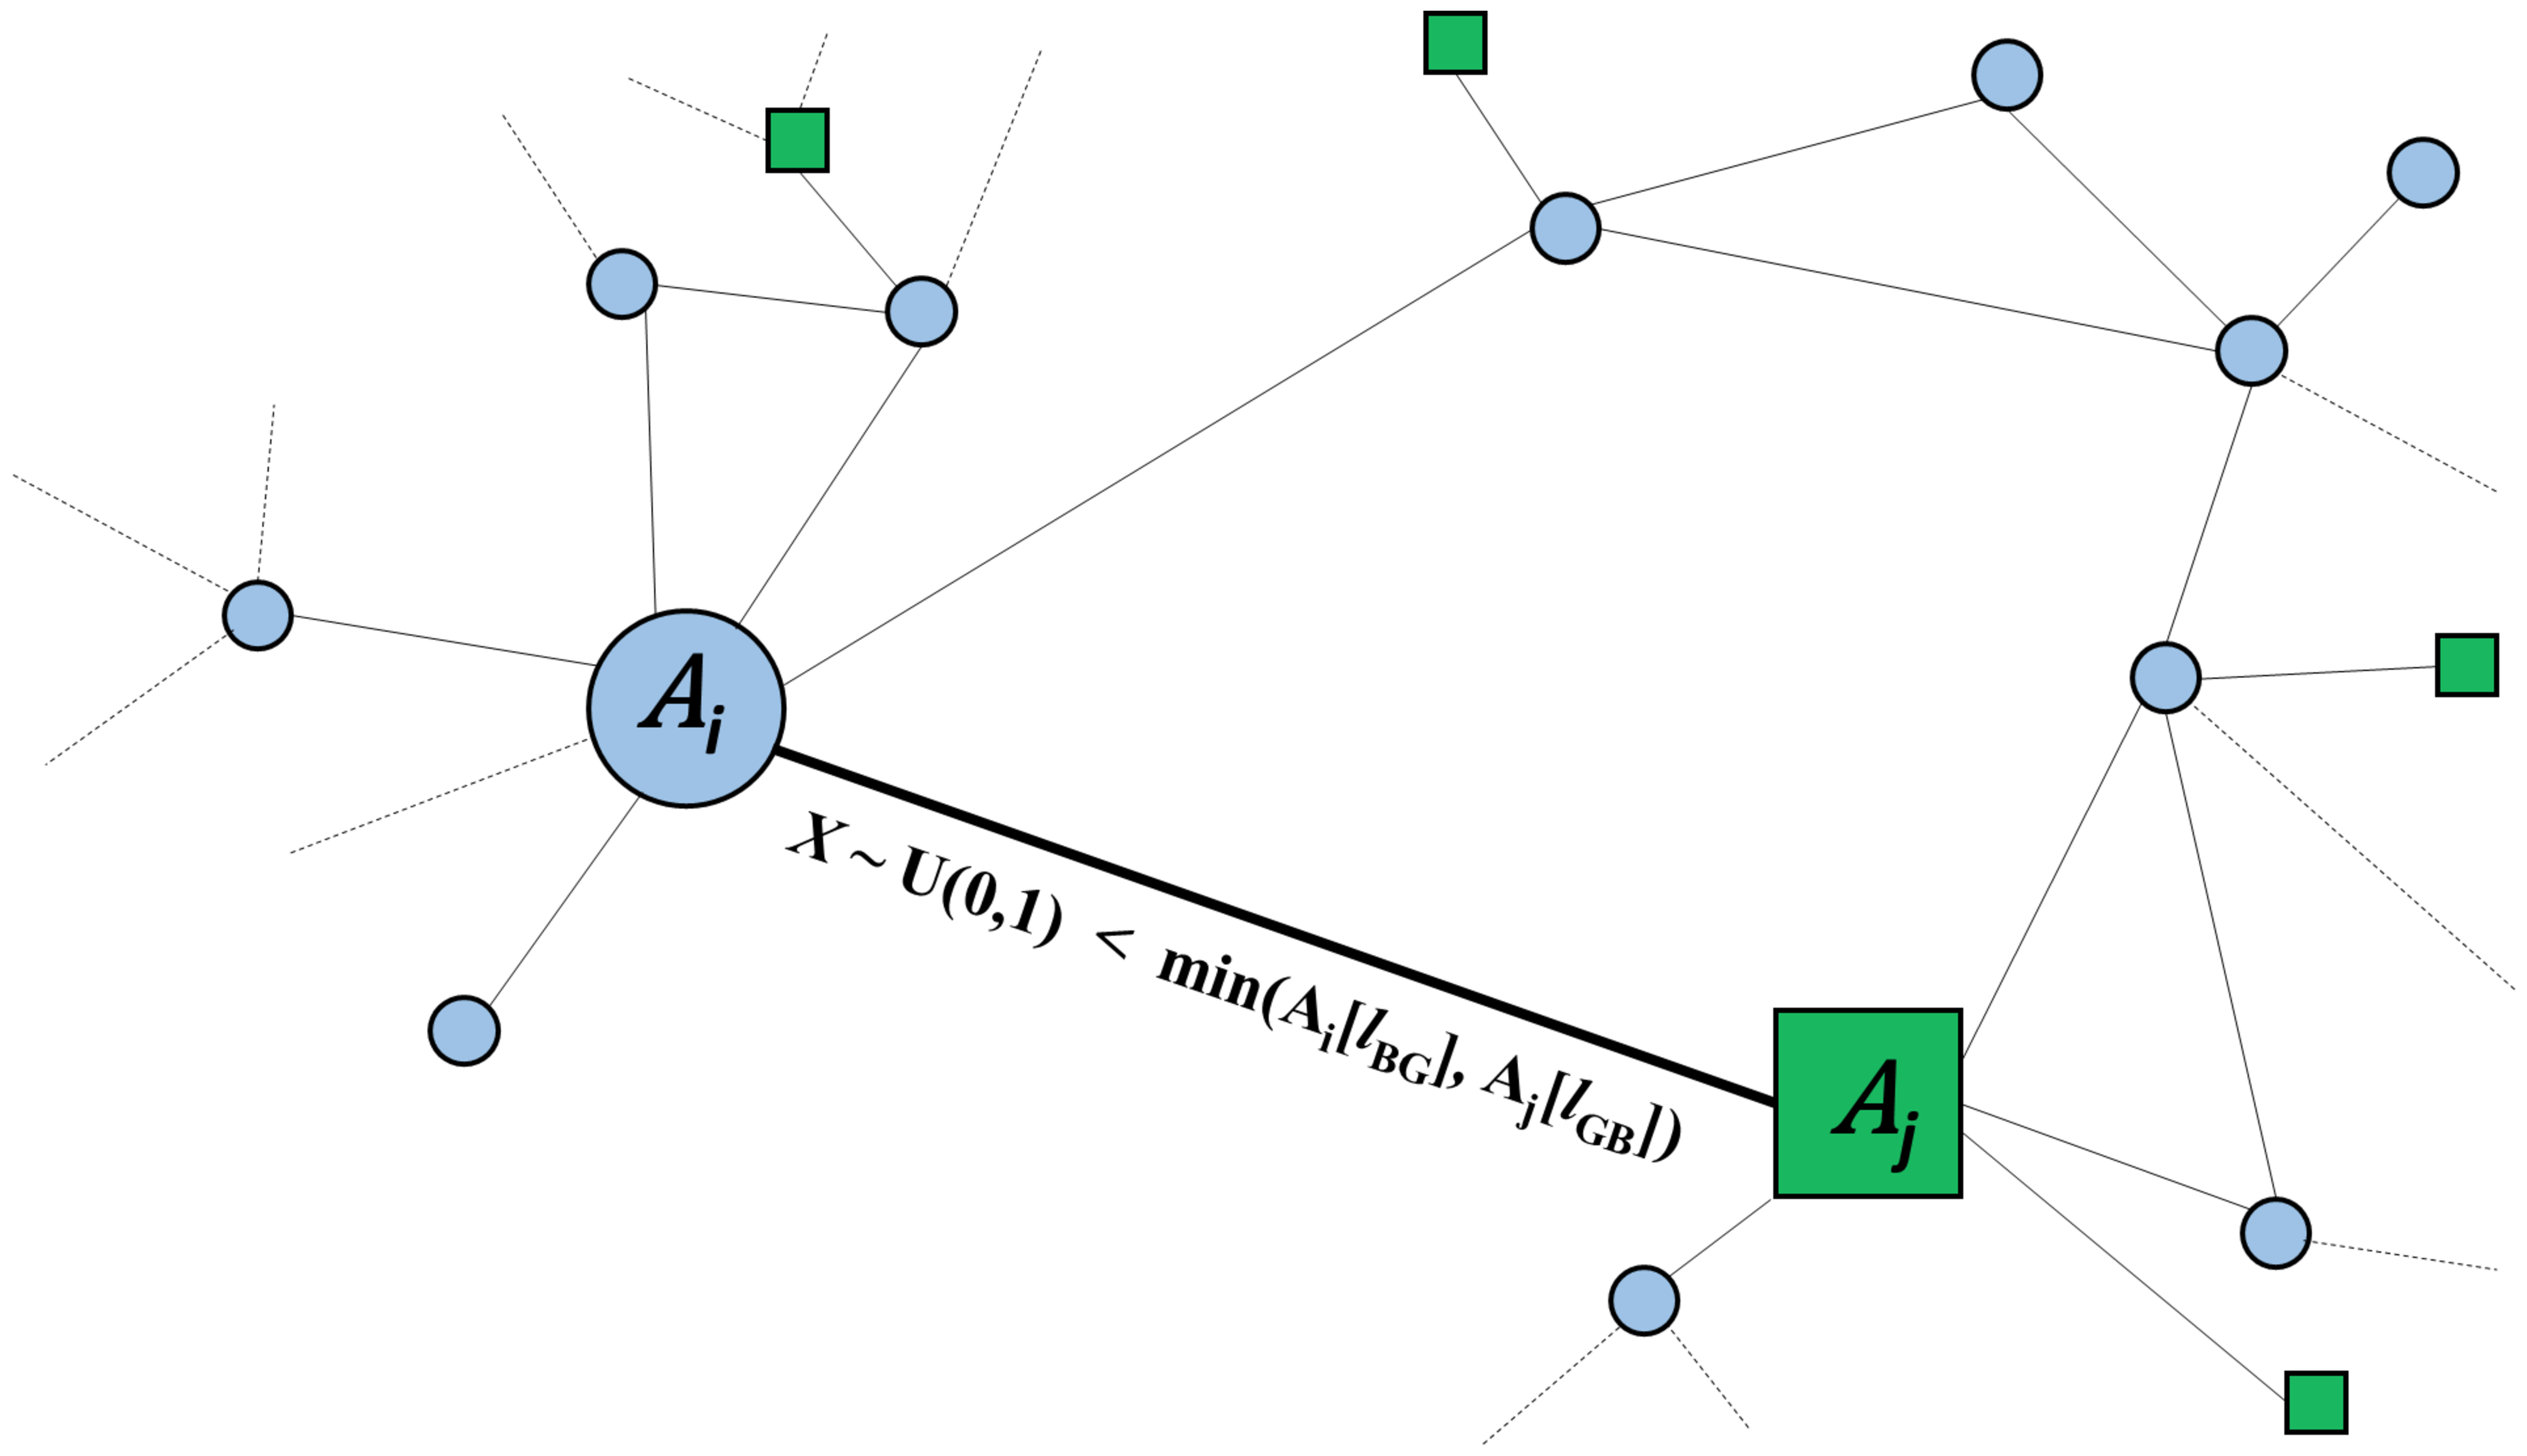
\includegraphics[width=1.0\linewidth]{figures/InteractionBarrier}
	\caption{Illustration sketch of the interaction barrier. Agents $ A_i $ and $ A_j $ interact pairwise. They will ``like'' each other with a probability proportional to the corresponding entry in the likeness matrix $ L $. If they succeed, then they will play a one-shot PD game.}
\end{figure}

For each agent pair, the group tag barrier is determined by the values of the agents' (heterogeneous) ``likenesses'' towards each other, as illustrated in figure 1. The two agents $ A_{i} $ and $ A_{j} $ will interact if  $ X \sim U(0,1) < \text{min}({A_{i}}_{[likenessOther]}, {A_{j}}_{[likenessOther]} ) $, where $ U(0,a) $ is the uniform distribution with support $ [0,a] $. Thus, the ``less friendly'' of the two agents (i.e. the one with smallest ``likeness'' towards the potential partner) will determine the maximum probability of successful interaction. Agents that have low ``likeness'' towards others can still interact, and agents with high ``likeness'' may not necessarily interact. Therefore, the group-tag barrier is applied with an element of randomness, which in this case represents the effect of noise in individual decisions (Skyrms and Pemantle 2000).

When two agents connected by a link are able to interact, they play a one-shot PD game whose payoff is communality. The PD was chosen instead of other social dilemma games (``Chicken run'' and ``Stag-hunt'') because it entails a stronger tension between full cooperation, ethnocentrism or purely greedy behavior than the other two games (Macy and Flache 2002). However, other types of games could easily be implemented in the model.

In the PD game agents can cooperate or defect according to the \texttt{groupTag} of the other agent and their individual strategies towards in- and out-group members. Using the standard notation, both agents receive communality $ R $ (reward payoff) or $ P $ (punishment payoff) if they both cooperate or defect, respectively. When one of the players defects and the other cooperates, the defector gets a communality $ T $ (temptation payoff) and the defector gets a communality $ S $ (sucker payoff). For the game to be a PD, the payoffs must verify the relationship $ T > R > P > S $ (Macy and Flache 2002). Since the payoff is expressed in an interval scale (i.e. the outcome of the game does not change if the payoff is subject to a linear map of the form $ y = a \cdot x + b  $, with $ a > 0 $ (Rapoport 1999)), we can set $ R = 1 $ and $ P = 0 $ without loss of generality. To further simplify the game, we set $ T = 1 + \gamma  $ and $ S = - \gamma $, where the parameter $ \gamma $ can the interpreted as a ``cooperation barrier'' (or ``strength'' of the game). In this way, the payoff matrix ($ M $) is
\begin{equation}
\label{eq:7}
M = \bordermatrix{~ & \texttt{C} & \texttt{D} \cr
	\texttt{C} & 1 & - \gamma \cr
	\texttt{D} & 1 + \gamma & 0 \cr}
\end{equation}
where the row labels are the strategies of the first player and the column labels those of the second player.

After agents play with all their link neighbors they try to improve their communality in the next round by either changing their strategy or their link neighbors. This process is modeled using an adaptation of the SPL model of cooperation in networks (Santos et al. 2006). Following Santos et al. (2006), at each time step agents revise their strategy $ \mathcal{S} $ or change their social ties, with relative frequency set by the input parameter $ W $. For $ W \to 0 $ the agents will have progressively higher inertia towards changing their social ties, whereas for large $ W $ they will react quickly to non-cooperative neighbors.
\begin{figure}[t!]
	\label{fig:StrategyUpdate}
	\centering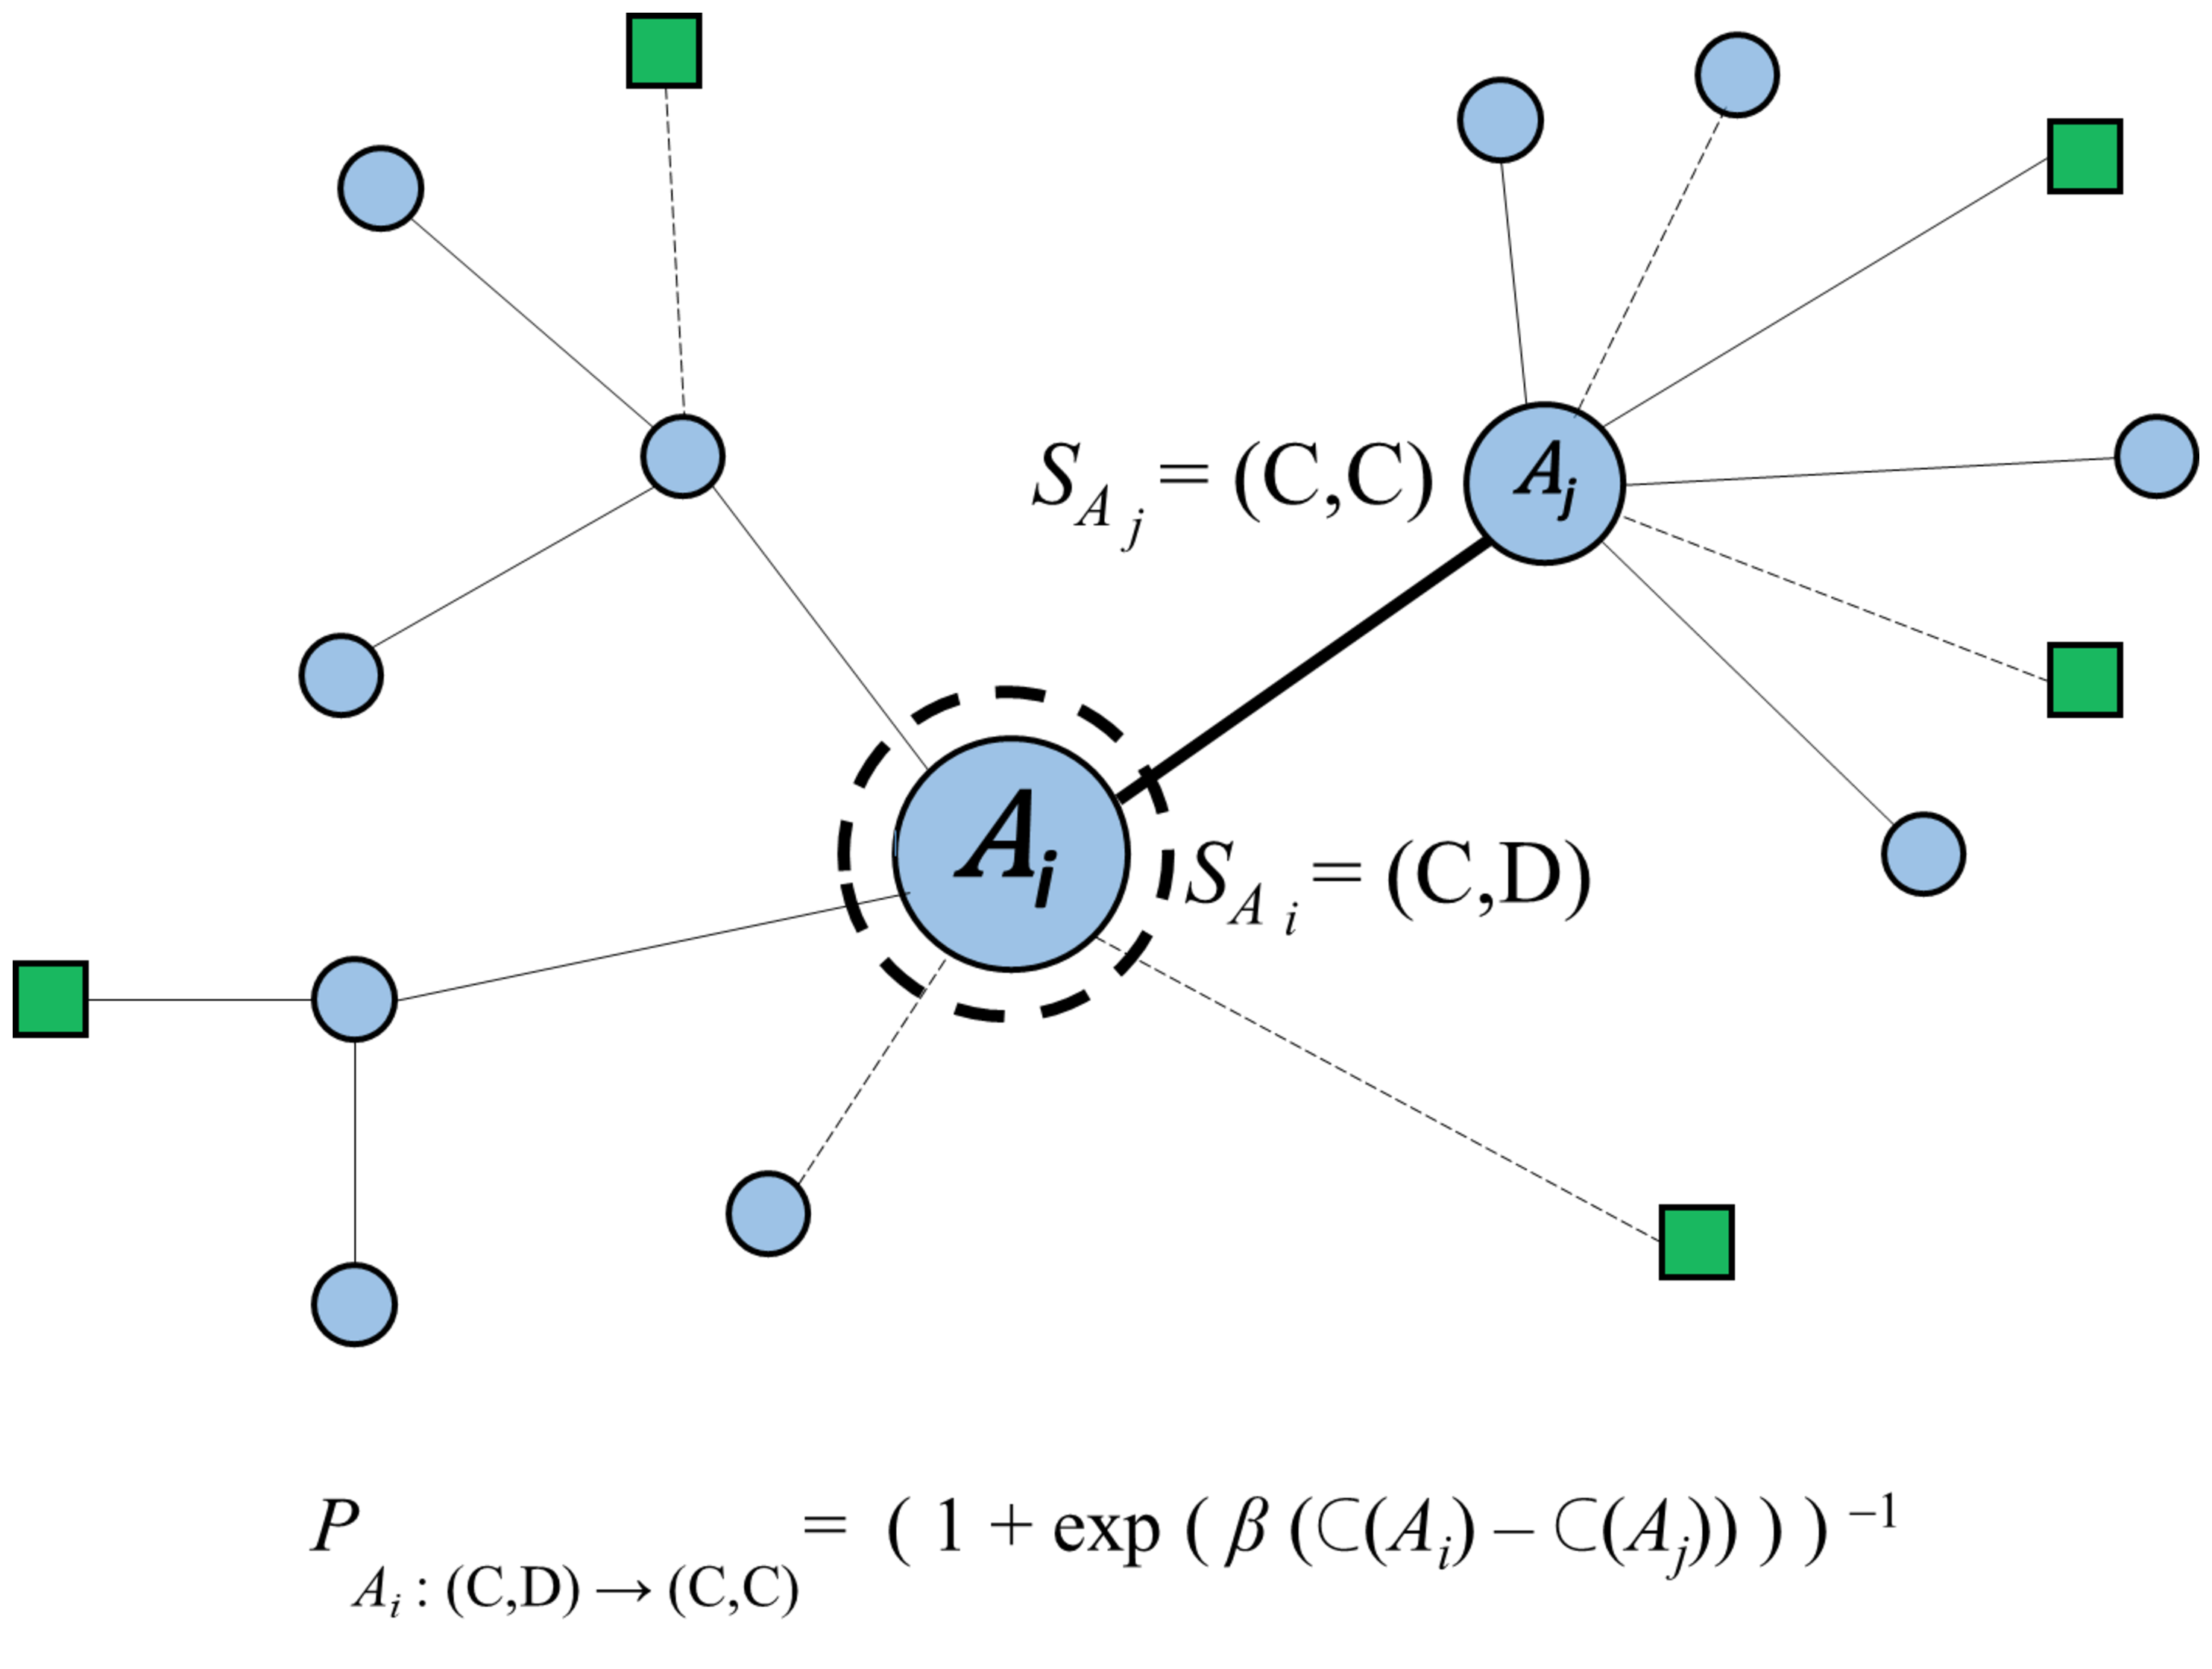
\includegraphics[width=0.85\linewidth]{figures/StrategyUpdate}
	\caption{Illustration sketch of the strategy update step. An agent $ A_i $ copies the strategy of the link neighbor that he ``likes'' and ``understands'' with largest communality ($ A_{j} $), with a probability given by a logistic function.}
\end{figure}



The process of strategy update for an agent $ A_{i} $ is sketched in figure 2. Agent $ A_{i} $ selects the link neighbor $ A_{j} $ with which it played the PD game (i.e. they ``liked'' each other in the last round of the game) with the larger number of link neighbors (maximum ``popularity''). Then, $ A_{i} $ imitates the strategy pair of $ A_{j} $ with probability $ P $ given by:
\begin{equation}
\label{eq:8}
P = \frac{1}{1 + \exp (\beta \cdot (\mathcal{C}(A_i) - \mathcal{C}(A_j))}
\end{equation}
where $ \beta = 0.005 $, $ \mathcal{C}(A_i) $ is the communality of $ A_i $ and $ \mathcal{C}(A_j) $ the communality of $ A_j $ (see Santos et al. (2006) for the foundation and details). 

\begin{figure}[t!]
	\label{fig:StructuralUpdate}
	\centering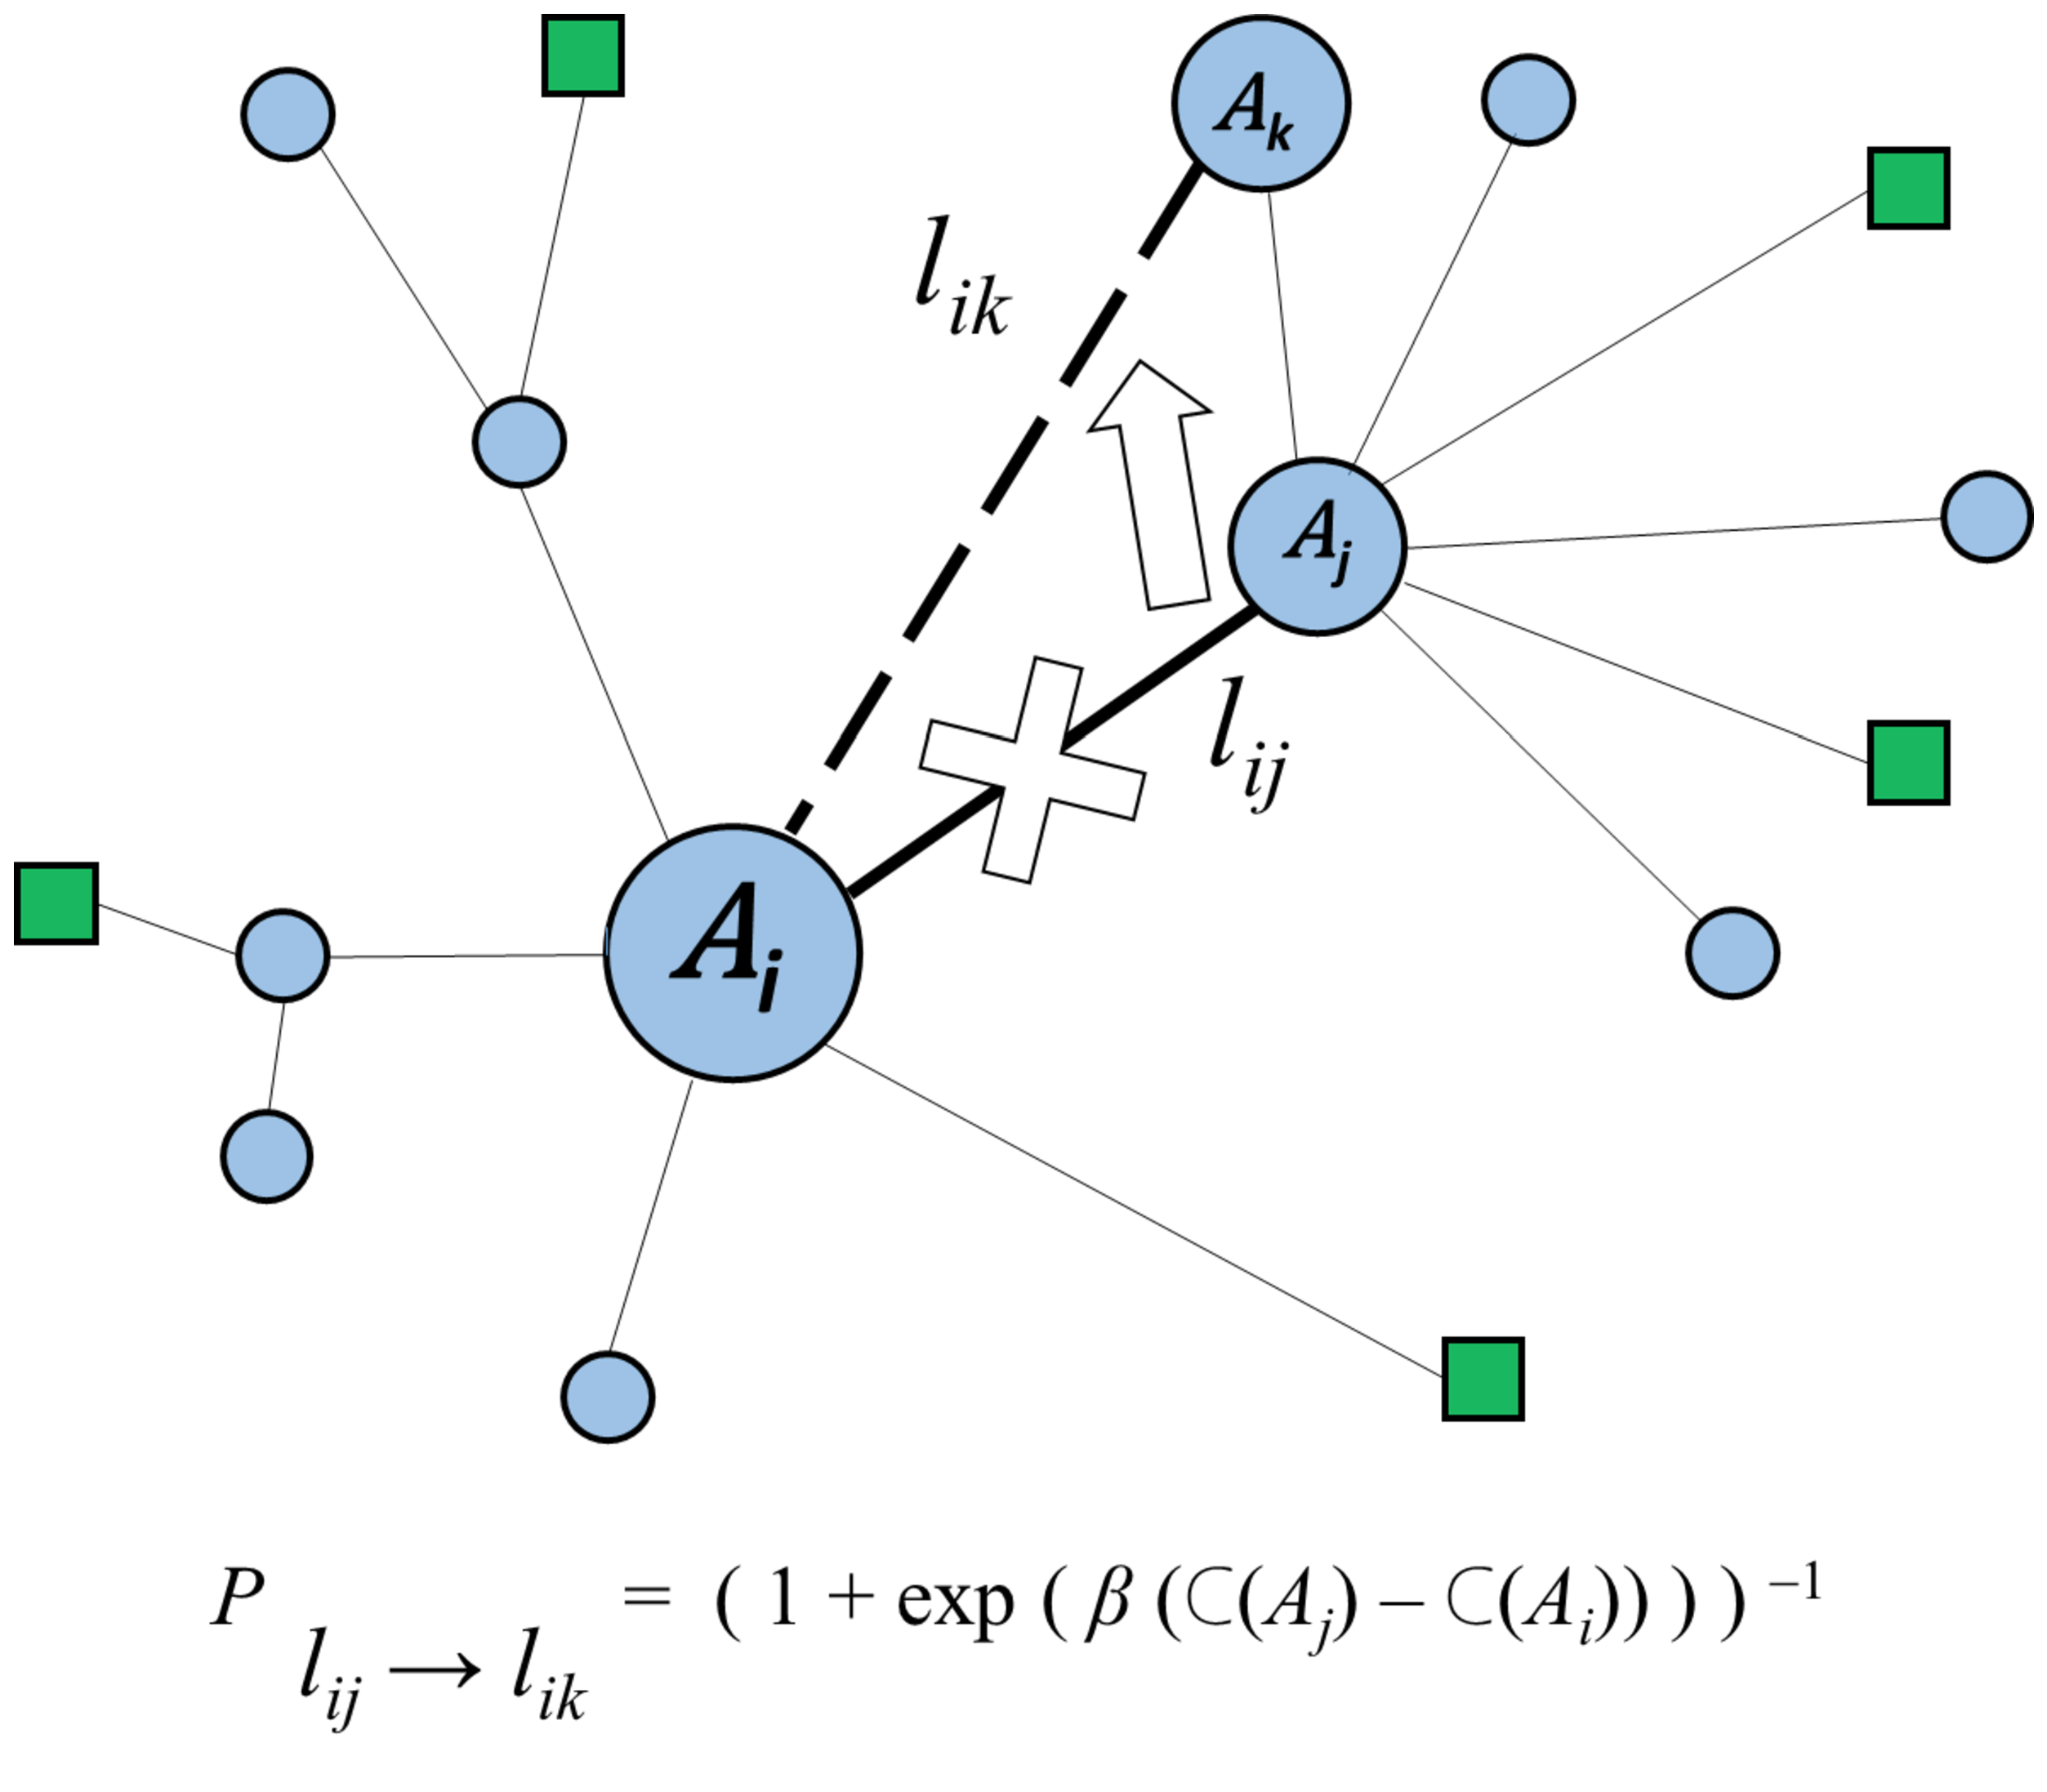
\includegraphics[width=0.75\linewidth]{figures/StructuralUpdate}
	\caption{Illustration sketch of the structural update. Agent $ A_i $ competes with agent $ A_j $ which is a defector, to create a link to agent $ A_k $ (link neighbor of $ A_j $).}
\end{figure}
Figure 3 illustrates the process of structural update for an agent $ A_i $. The agent picks at random one of its link neighbors $ A_j $ with more than one link. If in the last round $ A_j $ did not play with $ A_i $ or played and defected, then $ A_i $ will pick at random one of $ A_j $'s link neighbors, $ A_k $, and replace the link with $ A_j $ with a link to $ A_k $ with probability $ P $ given by (see Santos et al. (2006) for the foundation and details):
\begin{equation}
\label{eq:9}
P = \frac{1}{1 + \exp (\beta \cdot (\mathcal{C}(A_j) - \mathcal{C}(A_i))}
\end{equation}
where $ \beta = 0.005 $, $ \mathcal{C}(A_i) $ is the communality of $ A_i $ and $ \mathcal{C}(A_j) $ the communality of $ A_j $. This leads to agents severing social ties with defectors and agents they don't ``like'' or ``understand,'' and searching for cooperators among the link neighbors of the agents they want to get rid off. A link with another agent is not severed if it is the only link the other agent has, to ensure that the network remains connected. 


\subsection{Process Overview and Scheduling}
The model has two main procedures, \texttt{setup} and \texttt{go}. The \texttt{setup} procedure clears all variables from the previous simulation, initializes the global variables, creates the agents' list, and connects the agents in a small-world network with average node degree and rewiring probability given by $ n_{W} $ and rewiring probability $ p_{rewire} $, respectively (Watts and Strogatz 1998). For each agent, the \texttt{groupTag} attribute is randomly assigned with proportion determined by the $ P_{green} $ input parameter.

The initial strategies are assigned as follows. For each agent, the attributes \texttt{strategyOwn} and \texttt{strategyOther} are randomly assigned using the entries of the likeness matrix $ L $, as follows. For a generic agent $ A_i $, if $ \texttt{groupTag} (A_i) = \texttt{blue} $, the cooperation strategies towards in- and out-group members are assigned with probabilities
\begin{align}
\label{eq:10}
P(s_{in} (A_i) = C) & = l_{BB}  \\
P(s_{out} (A_i) = C) & =l_{BG}, 
\end{align}
and if $ \texttt{groupTag} (A_i) = \texttt{green} $ with probabilities
\begin{align}
\label{eq:11}
P(s_{in} (A_i) = C) & = l_{GG}  \\
P(s_{out} (A_i) = C) & = l_{GB}. 
\end{align}
In this way, the likeness matrix is used both for setting the barrier to successful interactions and initialization of the agents' strategies. This avoids introducing extra parameters for initialization and is easily extensible to cases with more than two groups.

The \texttt{go} procedure implements the model cycle. Each cycle consists of the following operations:
\begin{enumerate}
	\item Reset the agents' communality to 0.5;
	\item For each agent pair determine whether or not the agents will play a cooperation game. They will do so with a probability of liking  each other determined by the entries in the $ L $ matrix;
	\item Each agent pair with enough mutual ``likeness'' plays a PD game, and the agents' communality is updated depending on their respective strategy pairs;
	\item All agents individually decide to revise their strategies towards in- and out-group (social influence) or change its neighbors (social selection), depending on the input parameter $ W $;
	\item Increment the time cycle, and update the display if the model is run in interactive mode.
\end{enumerate}

\subsection{Validation, Parameterization and Calibration Issues}
We validated our model by observing, for different experiments, whether the results were coherent with fundamental anticipated outcomes summarized in Table \ref{tab:ExpectedEffect} below. For example, lower values of ``likeness'' and higher values of $ \gamma $ should invariably lead to difficulty of cooperation, and structural rigidity ($ W = 0 $) to impossibility of the network of mixed ties to grow, while producing plausible values for the variations of the emergent patterns of dominant strategies and network properties. Since our ABM is of ``abstract'' type parameterization and calibration were done by setting different experiments for characterizing the model's sensitivity to each parameter, comparing the impact of each parameter relative to the others, and finding parameter ranges that lead to sharp changes of the emergent patterns of dominant strategies for each group and the structure of the social network. 

\section{Results}
In this section, we present the results of four experiments for different combinations of the global variables that we expected to have the most significant effect on the model's behavior, as shown in Table \ref{tab:ExpectedEffect}. More specifically, the proportion of the minority group (\texttt{propGreen}) and the tag-induced barrier (\texttt{likeness}) are key variables in theories on intergroup conflict and cooperation (Allport 1958; Blalock 1967). The connectivity (\texttt{initialAverageNodeDegree}) is also a key parameter, as postulated by group contact theories (Allport 1958; Blumer 1958). Finally, the game strength (\texttt{gamma}) and the adaptivity (\texttt{W}) were shown to play a key role for describing cooperation in networks (Santos et al. 2006). In each experiment, four different global variables were swept simultaneously and the patterns of dominant strategy for each group and of the percentage of mixed ties were analyzed. The purpose of each experiment was to show whether the emergent patterns were coherent with the effects shown in Table \ref{tab:ExpectedEffect}, as well as the relative importance of each global variable on the model's behavior.   
\begin{table}[t!] \centering
	\small
	\begin{adjustbox}{width={\textwidth},totalheight={\textheight},keepaspectratio}%
	\begin{tabular}{ll}
		%\begin{tabularx}{\textwidth}{XXXX}
		\hline
		\textbf{Variable} & \textbf{Expected effect}  \\
		\hline
		\rule{0pt}{0ex} \texttt{propGreen} & full cooperation and \% of mixed ties increase with \% of   minority group\\ 
		\rule{0pt}{4ex} \texttt{initialAverageNodeDegree}  & full cooperation and \% of mixed ties increase with initial  connectivity\\ 
		\rule{0pt}{4ex} \texttt{likeness}   & difference of ``likeness'' towards in- and out-group influence whether \\
		&  in-group or full cooperation will prevail  \\
		\rule{0pt}{4ex} \texttt{gamma}  & increasing $ \gamma $ first induces defection towards group with smaller  \\
		& ``likeness'' and then full defection \\ 
		\rule{0pt}{4ex} \texttt{W} & increasing $ W $ promotes cooperation\\
		\hline
	\end{tabular}
\end{adjustbox}
	%\end{tabularx}
	\caption{Expected effect global variables on the model's behavior, with the remaining variables held constant.}
	
	\label{tab:ExpectedEffect}
\end{table}

Twenty simulations were performed for each of the 500 different combinations of the values of the input variables in all experiments. The results at the end of the simulations (500 cycles) were averaged over the twenty runs and represented in the form of facets plots.

\subsection{Experiment 1}
The purpose of this experiment was to study the effect of the combined variations of likeness towards in-group, likeness towards out-group, relative size of minority group ($ \mathcal{G}_{\mathcal{S}} $) and initial average connectivity ($ n_{W} $), keeping the game barrier ($ \gamma $) and frequency of strategy updates ($ W $) constant. The likeness towards in- and out-group was set equal for both groups (i.e. $ l_{BB} = l_{GG} $ and $ l_{GB} = l_{BG} $).
\begin{table}[t!] \centering
	\small
	\begin{tabular}{ll}
		%\begin{tabularx}{\textwidth}{XXXX}
		\hline
		\textbf{Variable} & \textbf{Range/Values}    \\
		\hline
		\rule{0pt}{0ex} \texttt{numAgents}  & 1000 \\
		\rule{0pt}{4ex} \texttt{numCycles} & 500  \\                    
		\rule{0pt}{4ex} \texttt{propGreen} &  \{0.1,0.15,0.20,0.25,0.30\} \\
		\rule{0pt}{4ex} \texttt{initialAverageNodeDegree}  & \{8,12,16,20\}    \\
		\rule{0pt}{4ex} \texttt{pRewire} & 0.25 \\
		\rule{0pt}{4ex} \texttt{gamma} & 2 \\
		\rule{0pt}{4ex} \texttt{W} & 5 \\
		\rule{0pt}{4ex} $  $$ \texttt{likeness}_{BB} $   &  \{0.0,0.25,0.50,0.75,1.00\} \\
		\rule{0pt}{4ex} $ \texttt{likeness}_{GG} $   &   $ = \texttt{likeness}_{BB} $\\
		\rule{0pt}{4ex} $ \texttt{likeness}_{BG} $   &  \{0.0,0.25,0.50,0.75,1.00\} \\
		\rule{0pt}{4ex} $ \texttt{likeness}_{GB} $   &   $ = \texttt{likeness}_{BB} $\\
		\hline
	\end{tabular}
	%\end{tabularx}
	\caption{Default values of the input variables for experiments reported in this work. These values are common to all experiments, unless stated otherwise.}
	\label{tab:Experiment1}
\end{table}


\begin{figure}[t!]
	\label{fig:strategyHostExperiment1}
	%\centering
	\begin{minipage}[c]{0.2\linewidth}
		\caption{Facets plot of the dominant strategy within the ``blue'' (majority) population after 500 cycles, obtained in experiment 1.}
	\end{minipage}
	\begin{minipage}[c]{0.75\linewidth}
		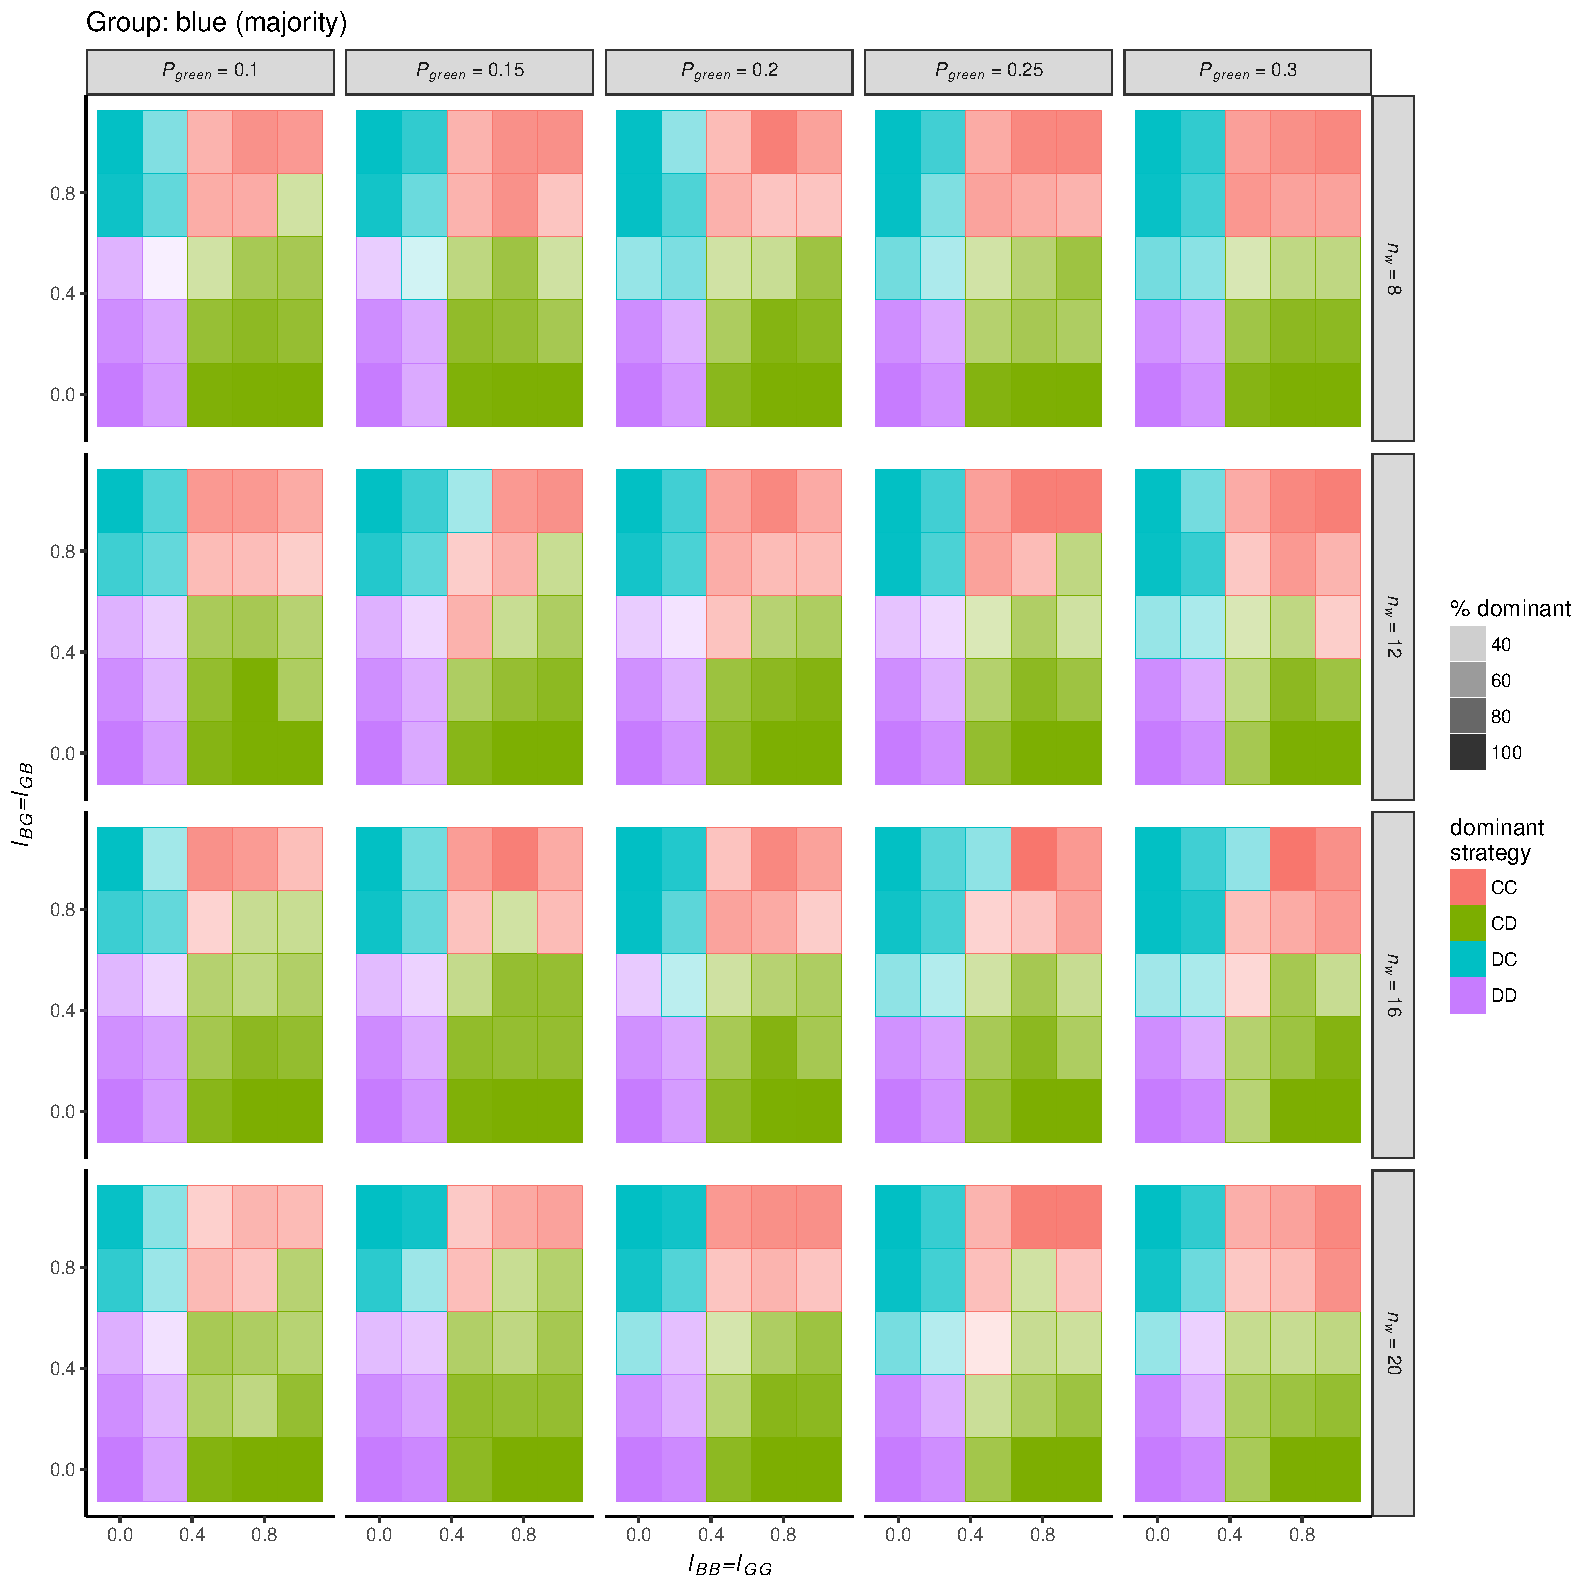
\includegraphics[trim={0cm 0cm 0.4cm 0cm}, clip, width=\linewidth]{figures/strategyHostExperiment1.pdf}
	\end{minipage}
\end{figure}

Figures 4 and 5 show the facets plots of the dominant strategies within the ``blue'' and ``green'' populations, respectively, at the end of each run (500 cycles) and averaged over twenty runs. In these plots, each of the four possible strategies is represented by a different color. Because not all agents have the same strategy at the end of the simulations, the \% of the agents that have the dominant strategy is represented using a transparency $ \alpha $ scale.

The first aspect to notice is that there is virtually no difference between these two plots. This was to be expected in this case, since the ``likenesses'' towards in- and out-group were identical for both populations. Therefore, in subsequent experiments where this condition holds, only the plots for the dominant strategy of the majority group will be shown. Although the plots show the dominant strategies, the shadings of each small tile show that in many cases other strategies were also present within the two groups.
\begin{figure}[t!]
	\label{fig:strategyImmigrantExperiment1}
	%\centering
	\begin{minipage}[c]{0.2\linewidth}
		\caption{Facets plot of the dominant strategy within the ``green'' (minority) population after 500 cycles, obtained in experiment 1.}
	\end{minipage}
	\begin{minipage}[c]{0.75\linewidth}
		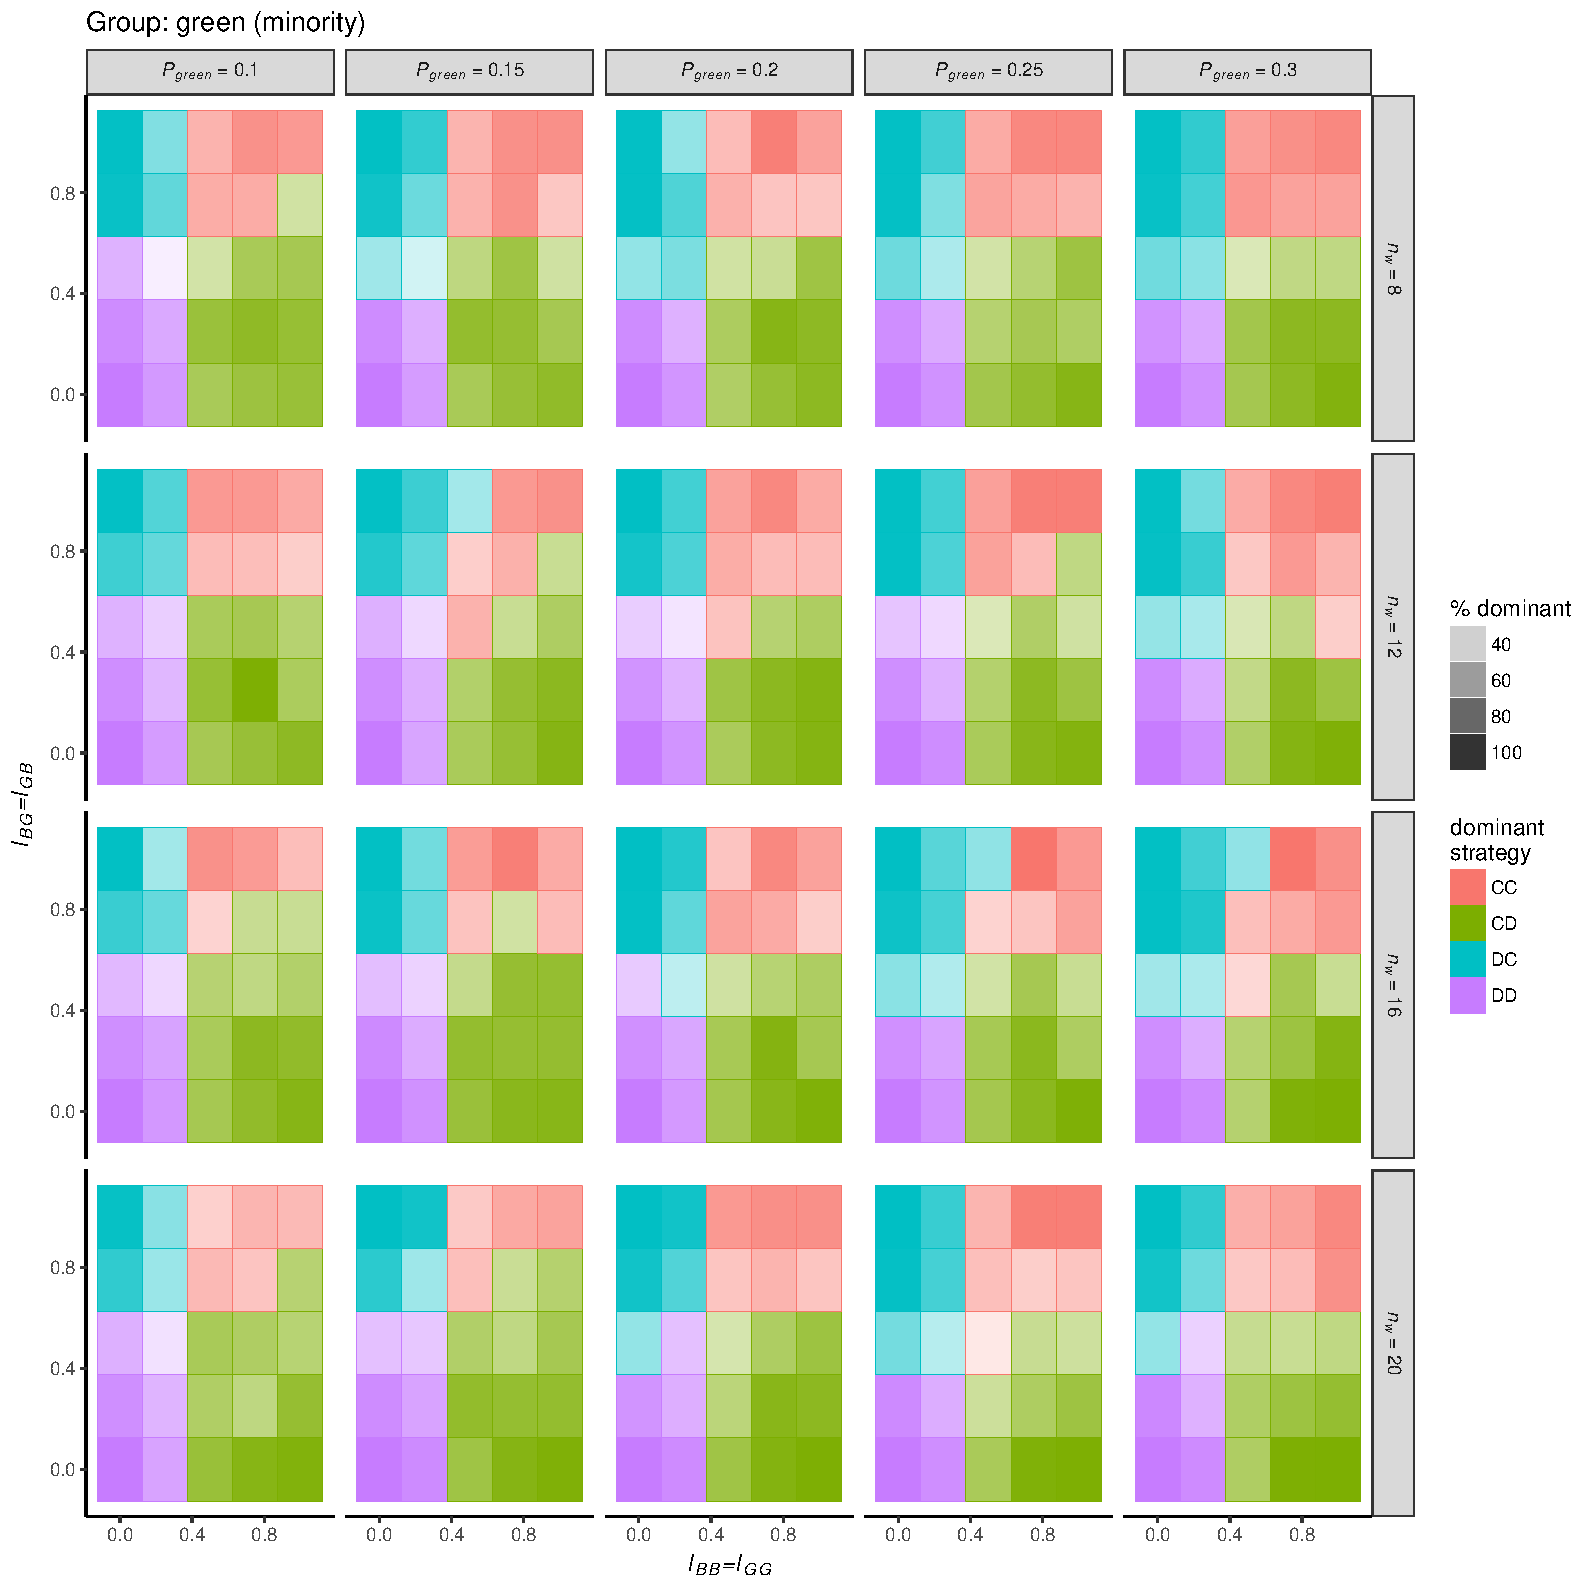
\includegraphics[trim={0cm 0cm 0.4cm 0cm}, clip, width=\linewidth]{figures/strategyImmigrantExperiment1.pdf}
	\end{minipage}
\end{figure}

Another aspect to notice that all the four strategies can come out as dominant, depending on the relative values of the ``likeness'' towards in- and out-group. The point in the \{\texttt{likenessOwn}, \texttt{likenessOther}\} plane which seems to divide the regions where each strategy dominates is strongly dependent on these two ``likenesses'' but is relatively insensitive to the relative size of the minority group and the initial average node degree.
\begin{figure}[ht!]
	\label{fig:avgBlueAgentDegreeExperiment1}
	%\centering
	\begin{minipage}[c]{0.2\linewidth}
		\caption{Facets plot of the average node degree (number of link neighbors) for the ``blue'' (majority) population after 500 cycles, obtained in experiment 1.}
	\end{minipage}
	\begin{minipage}[c]{0.75\linewidth}
		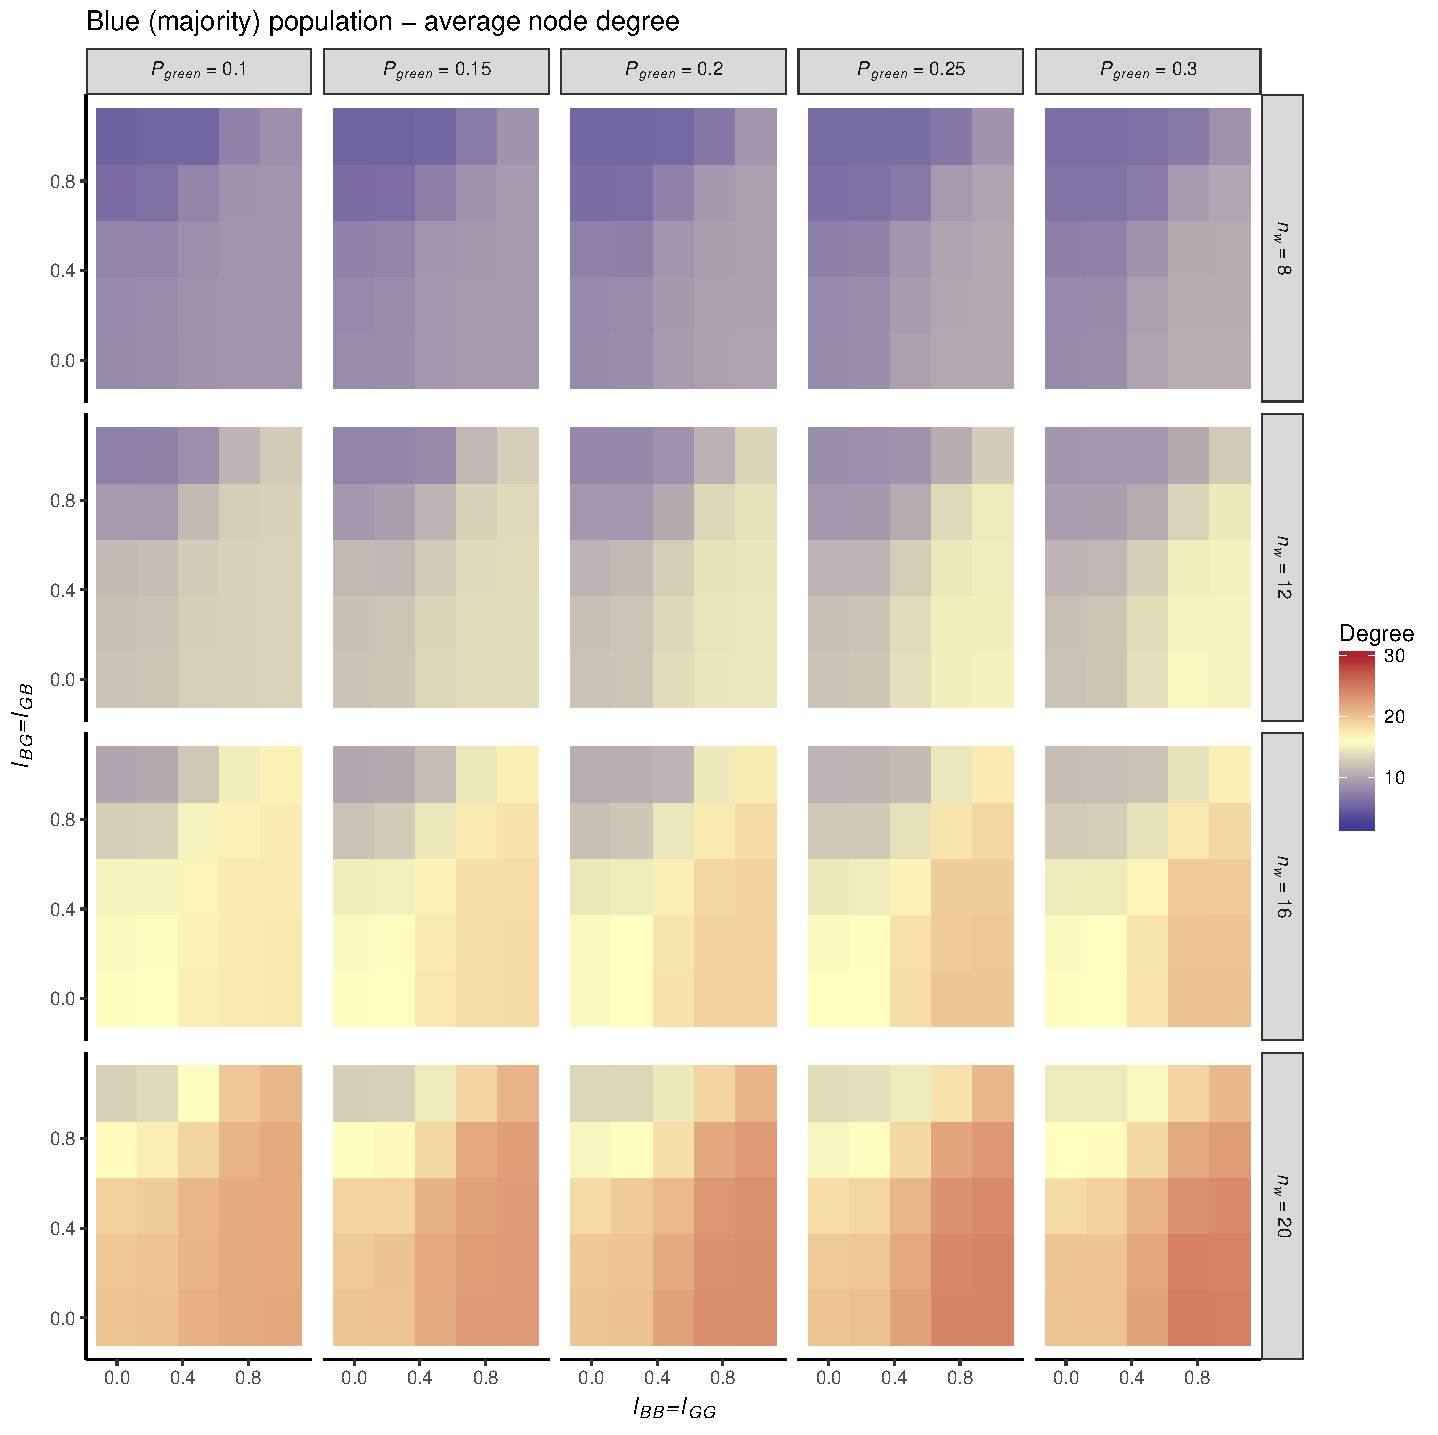
\includegraphics[trim={0cm 0cm 0.4cm 0cm}, clip, width=\linewidth]{figures/avgBlueAgentDegreeExperiment1.pdf}
	\end{minipage}
\end{figure}

Figures 6 and 7 show the average node degree for the ``blue'' and ``green'' populations, respectively. By observing the color values corresponding to each value of $ n_{W} $ in the facets plot in figure 6, it is apparent that the average node degree at the end of the simulations is clearly dependent on the initial average node degree. Thus, the relative size of the minority group has a weaker influence on the \% of mixed ties than the initial degree of connectivity. This is consistent with Blau's macro-sociological theory of social structure, according to which the degree of connectivity is the major structural factor influencing intergroup relations (Blau 1977). Also, the average node degree increases with the ``likeness'' towards in-group and decreases with the ``likeness'' towards the out-group, as was expected from the arguments in Table \ref{tab:ExpectedEffect}.
\begin{figure}[ht!]
	\label{fig:avgGreenAgentDegreeExperiment1}
	%\centering
	\begin{minipage}[c]{0.2\linewidth}
		\caption{Facets plot of the average node degree (number of link neighbors) for the ``green'' (minority) population after 500 cycles, obtained in experiment 1.}
	\end{minipage}
	\begin{minipage}[c]{0.75\linewidth}
		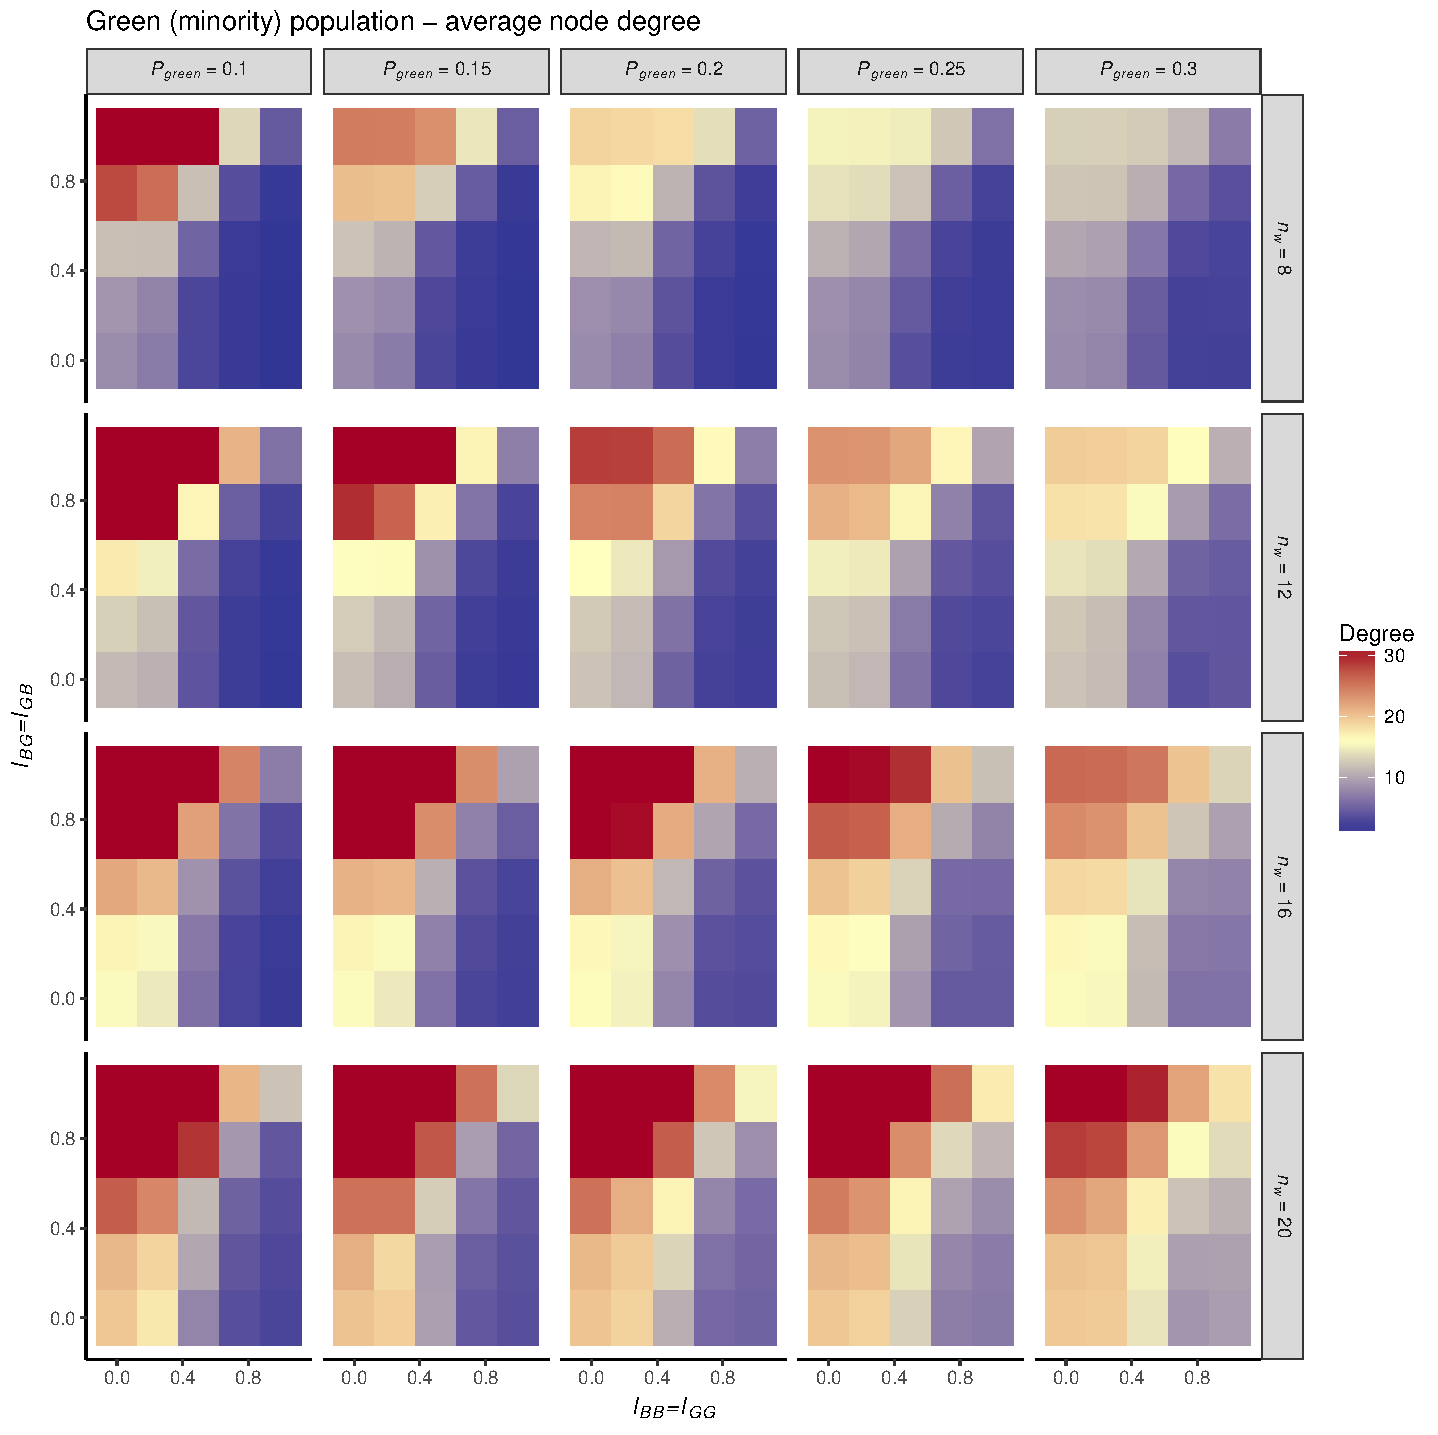
\includegraphics[trim={0cm 0cm 0.4cm 0cm}, clip, width=\linewidth]{figures/avgGreenAgentDegreeExperiment1.pdf}
	\end{minipage}
\end{figure}

The facets plot of the average node degree of the ``green'' population in figure 7 shows a qualitatively different behavior than that depicted in figure 6. Since the color scales are the same in both figures, it is observed that when the ``likeness'' towards the out-group is larger than the ``likeness'' towards the in-group (upper left corners in each heat map) the minority group ends up with a larger average node degree than the majority group. Also, the average node degree of the minority group is strongly dependent on all four sweeping variables.

The conditions leading to larger average node degree for the minority also lead to smaller average node degree of the majority. One interesting aspect to notice is that the average node degree increases with the ``likeness'' towards out-group and decreases with the ``likeness'' towards in-group, which is the reverse of the result for the majority population. Also, for low values of $ l_{GG} $ and high values of $ l_{GB} $  the node degree increases for decreasing size of the minority group. Thus, according to our model, agents belonging to a minority group can get a larger average connectivity than a majority group, by having a significantly higher ``likeness'' towards the out-group than towards the in-group. 
\begin{figure}[ht!]
	\label{fig:pctMixedTiesExperiment1}
	%\centering
	\begin{minipage}[c]{0.2\linewidth}
		\caption{Facets plot of the percentage of mixed ties (links between agents of different groups) after 500 cycles, obtained in experiment 1.}
	\end{minipage}
	\begin{minipage}[c]{0.75\linewidth}
		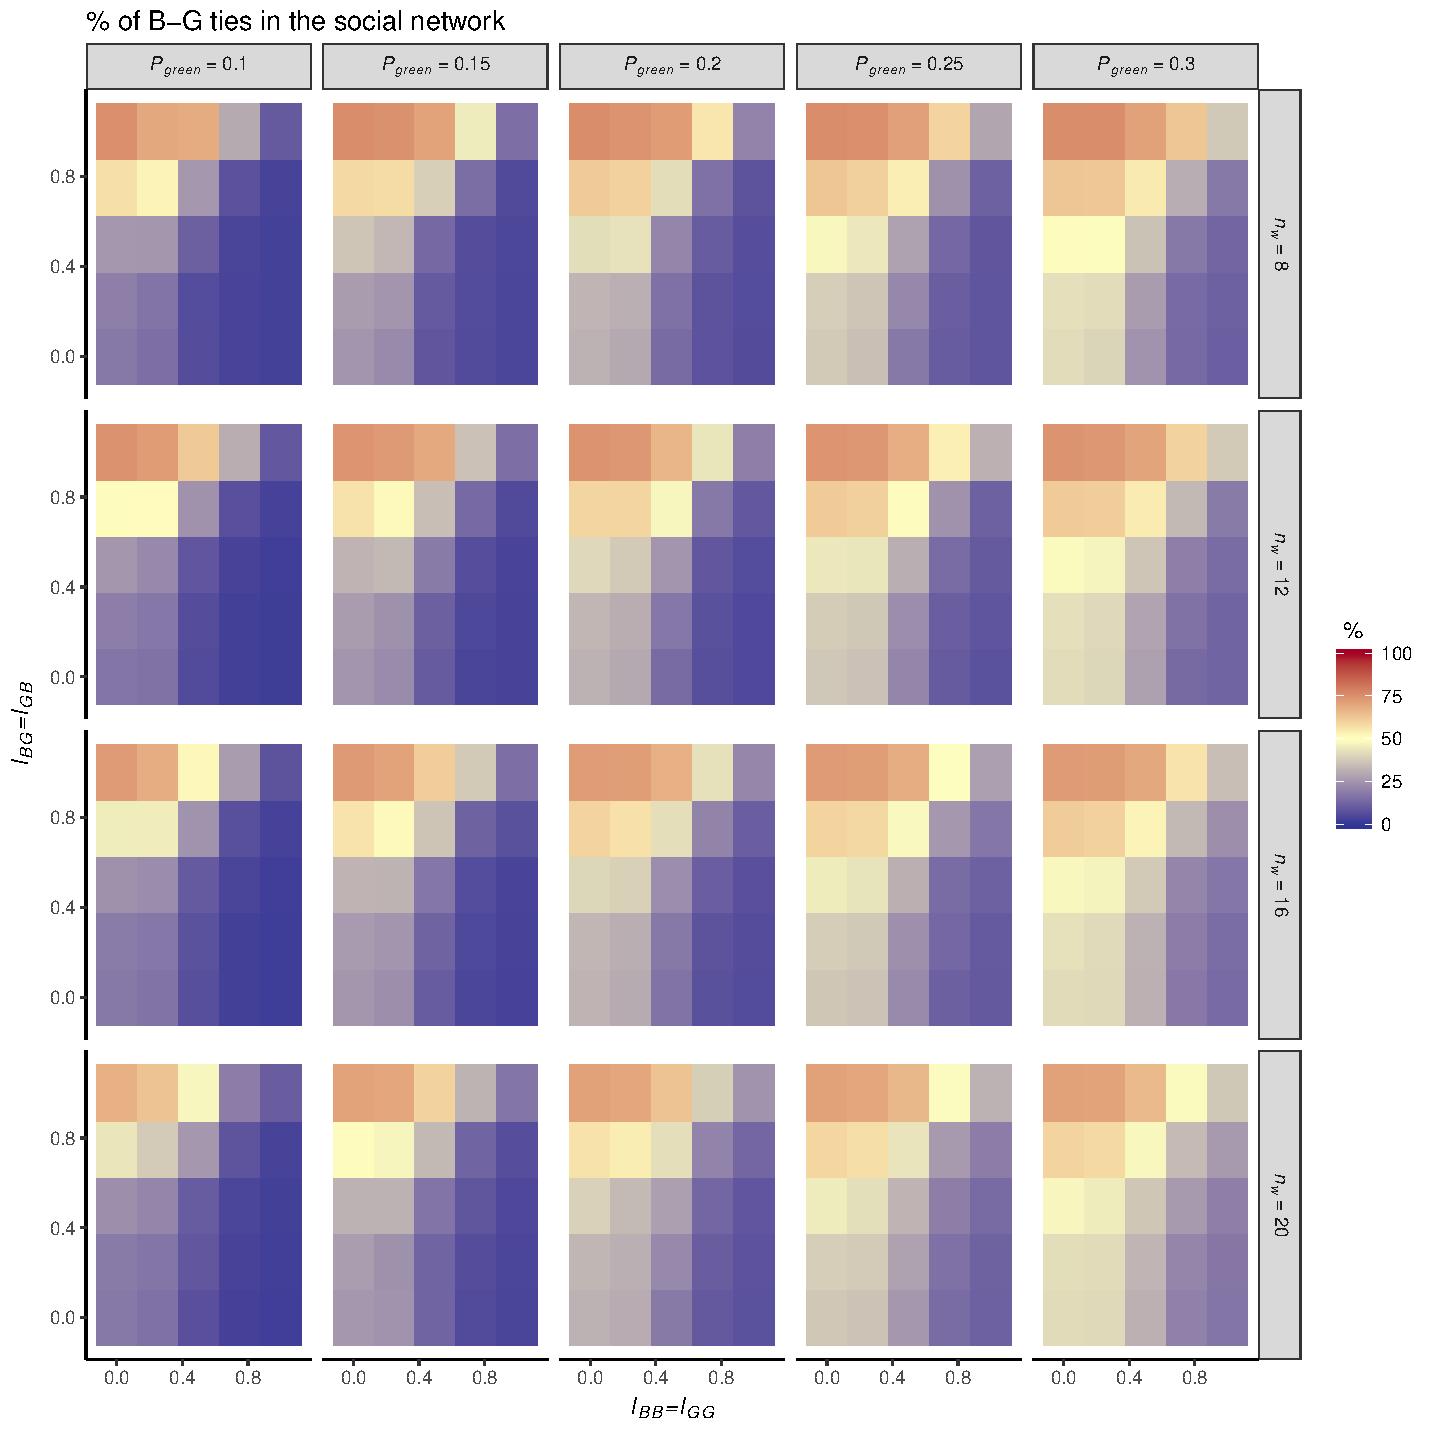
\includegraphics[trim={0cm 0cm 0.4cm 0cm}, clip, width=\linewidth]{figures/pctMixedTiesExperiment1.pdf}
	\end{minipage}
\end{figure}

Figure 8 shows the percentage of the mixed ties (i.e. those with agents belonging to different groups) in the social network. The results show that the formation of a network of mixed ties requires high `'likeness'' towards the out-group and low ``likeness'' towards the in-group, as was expected (based on the arguments in table \ref{tab:ExpectedEffect}). This result is consistent with the findings by McPherson et al. (2001). The increasing relative size of the minority group also promotes the formation of mixed ties. This too was expected, for the increasing percentage of the minority group within the mixed population increases the initial probability of interaction between agents belonging to different groups. The influence of the initial degree of connectivity is weaker than that of the relative size of the minority group.


\subsection{Experiment 2}
The purpose of this experiment was to study the effect of the combined variations of likeness towards in-group, likeness towards out-group, relative size of minority group $ \mathcal{G}_{\mathcal{S}} $ and $ W $ (which controls adaptivity), keeping the initial average connectivity $ n_{W} $, and  $ \gamma $ constant. More specifically, we were interested in determining whether the relative size of the minority group has a stronger influence on the qualitative behavior of the solutions or vice-versa.

The initial average node degree was set at the constant value $ n_W = 16 $. The sweeping variables were the size of the minority group and the ``likenesses,'' which were set as in experiment 1, and the frequency of structural to strategy updates, which was set $ W = \{0,1,5,10\} $.
\begin{figure}[ht!]
	\label{fig:strategyHostExperiment2}
	%\centering
	\begin{minipage}[c]{0.2\linewidth}
		\caption{Facets plot of the dominant strategy within the ``blue'' (majority) population after 500 cycles, obtained in experiment 2.}
	\end{minipage}
	\begin{minipage}[c]{0.75\linewidth}
		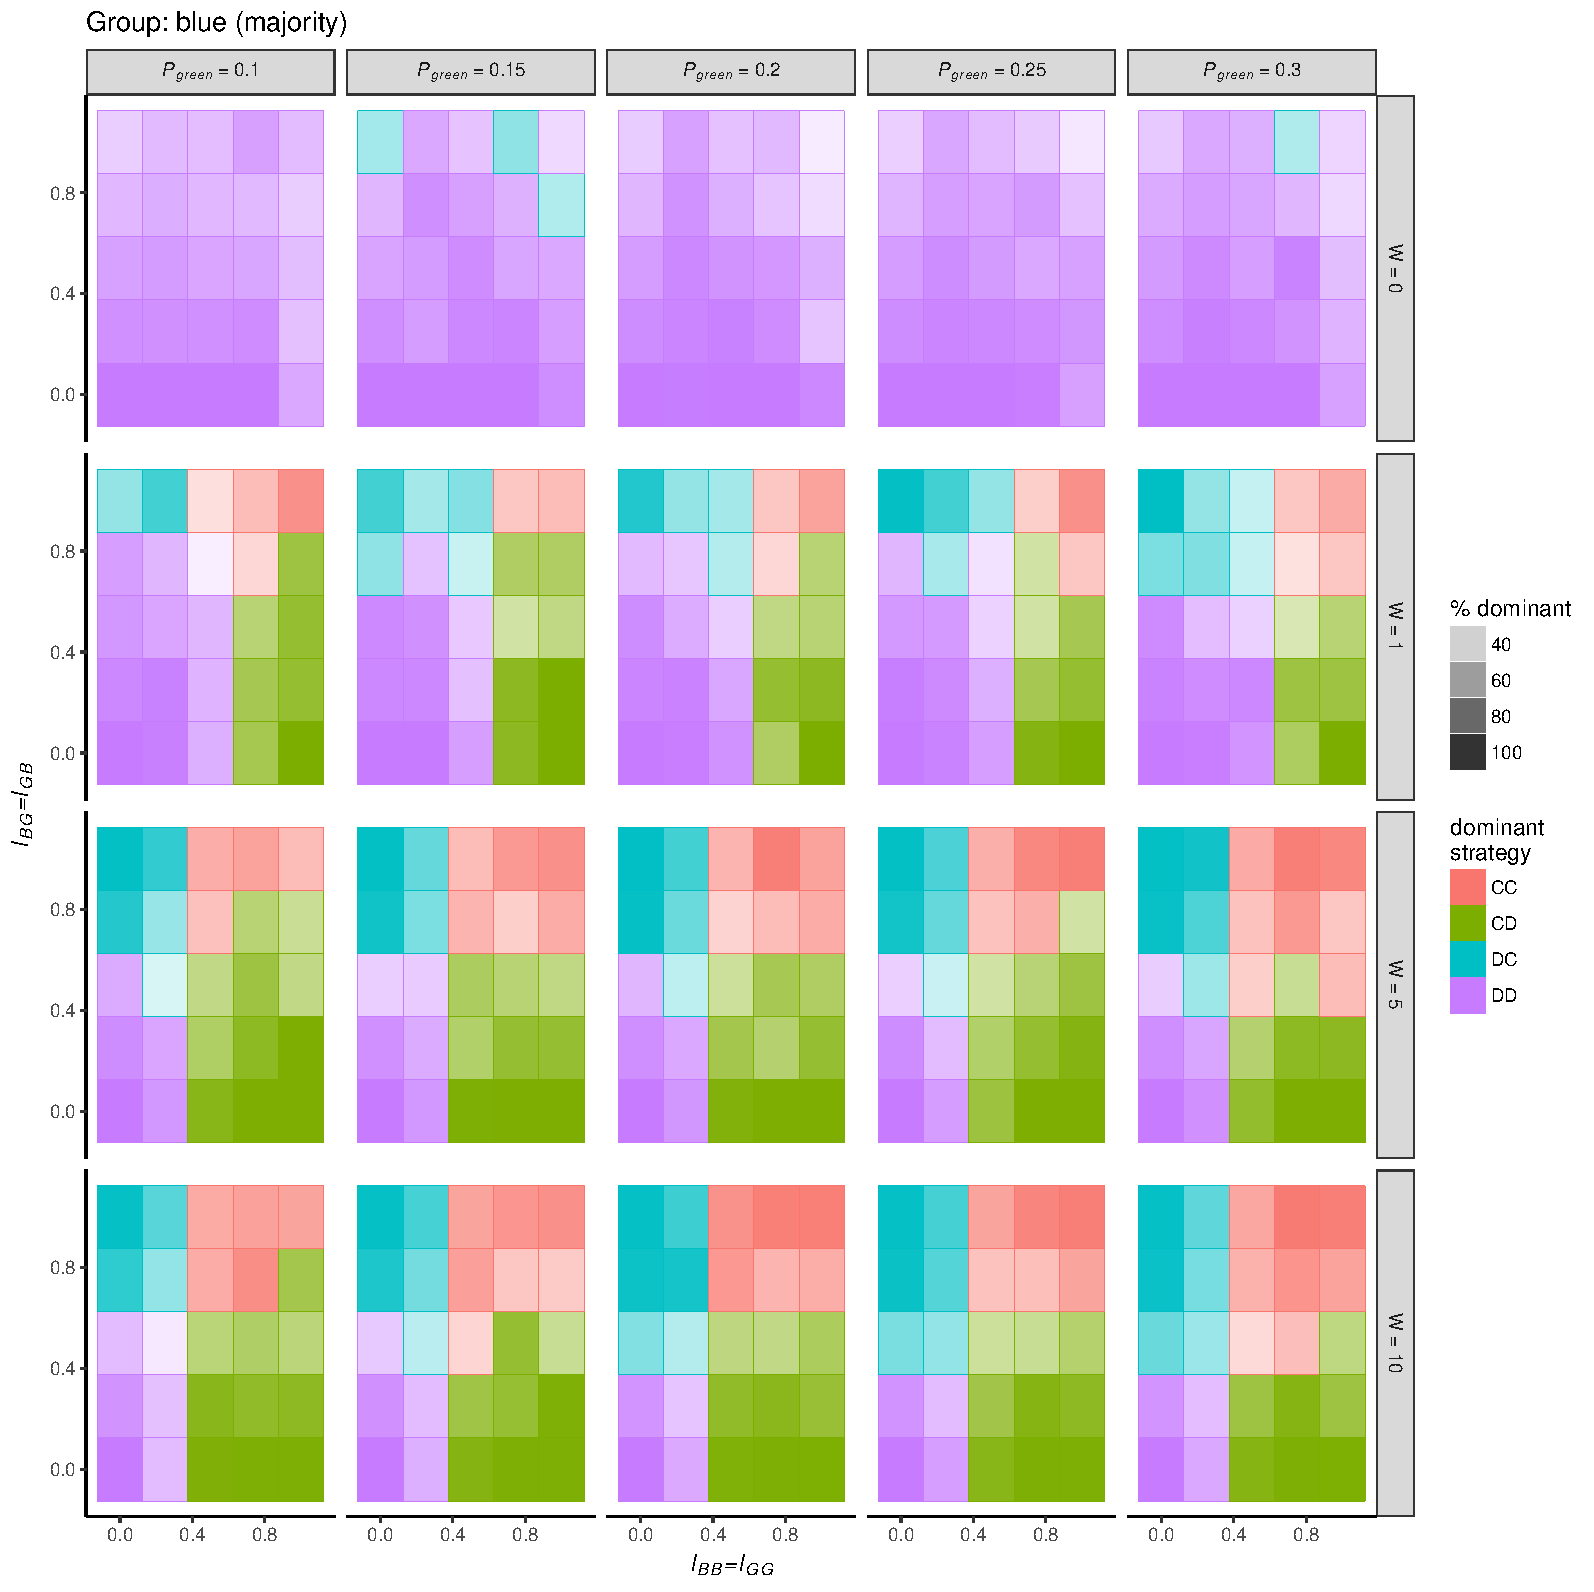
\includegraphics[trim={0cm 0cm 0.4cm 0cm}, clip, width=\linewidth]{figures/strategyHostExperiment2.pdf}
	\end{minipage}
\end{figure}

Figures 9 and 10 show the facets plots of the dominant strategy for the ``blue'' (majority) population and the percentage of mixed ties in the social network, respectively, at the end of each run (500 cycles) and averaged over twenty runs. These results confirm the well-known fact that adaptivity plays a key role for promoting cooperation in networks (Santos et al. 2006; Santos et al. 2006a). If the network is kept rigid ($ W = 0 $), the dominant strategy is full defection (\texttt{DD}) for almost all pairs of values of the ``likenesses'' and mixed ties do not form. For slow adaptivity ($ W =1 $), the dominant strategy is full defection except for relatively high values of $ l_{BB} = l_{GG}$ and $ l_{BG} = l_{GB}$, which is consistent with the general theory of the PD game (Macy and Flache 2002; Dixit et al. 2015; Santos et al. 2006). For $ W \geq 1 $ the transitions from ethnocentric behavior (dominant \texttt{CD}) to full cooperation are determined by the ``likeness'' towards the out-group. Analysis of figures 9 and 10  also suggests that adaptivity has a stronger influence on the resulting dominant strategies than the relative size of the minority group.
\begin{figure}[t!]
	\label{fig:pctMixedTiesExperiment2}
	%\centering
	\begin{minipage}[c]{0.2\linewidth}
		\caption{Facets plot of the percentage of mixed ties (links between agents of different groups) after 500 cycles, obtained in experiment 2.}
	\end{minipage}
	\begin{minipage}[c]{0.75\linewidth}
		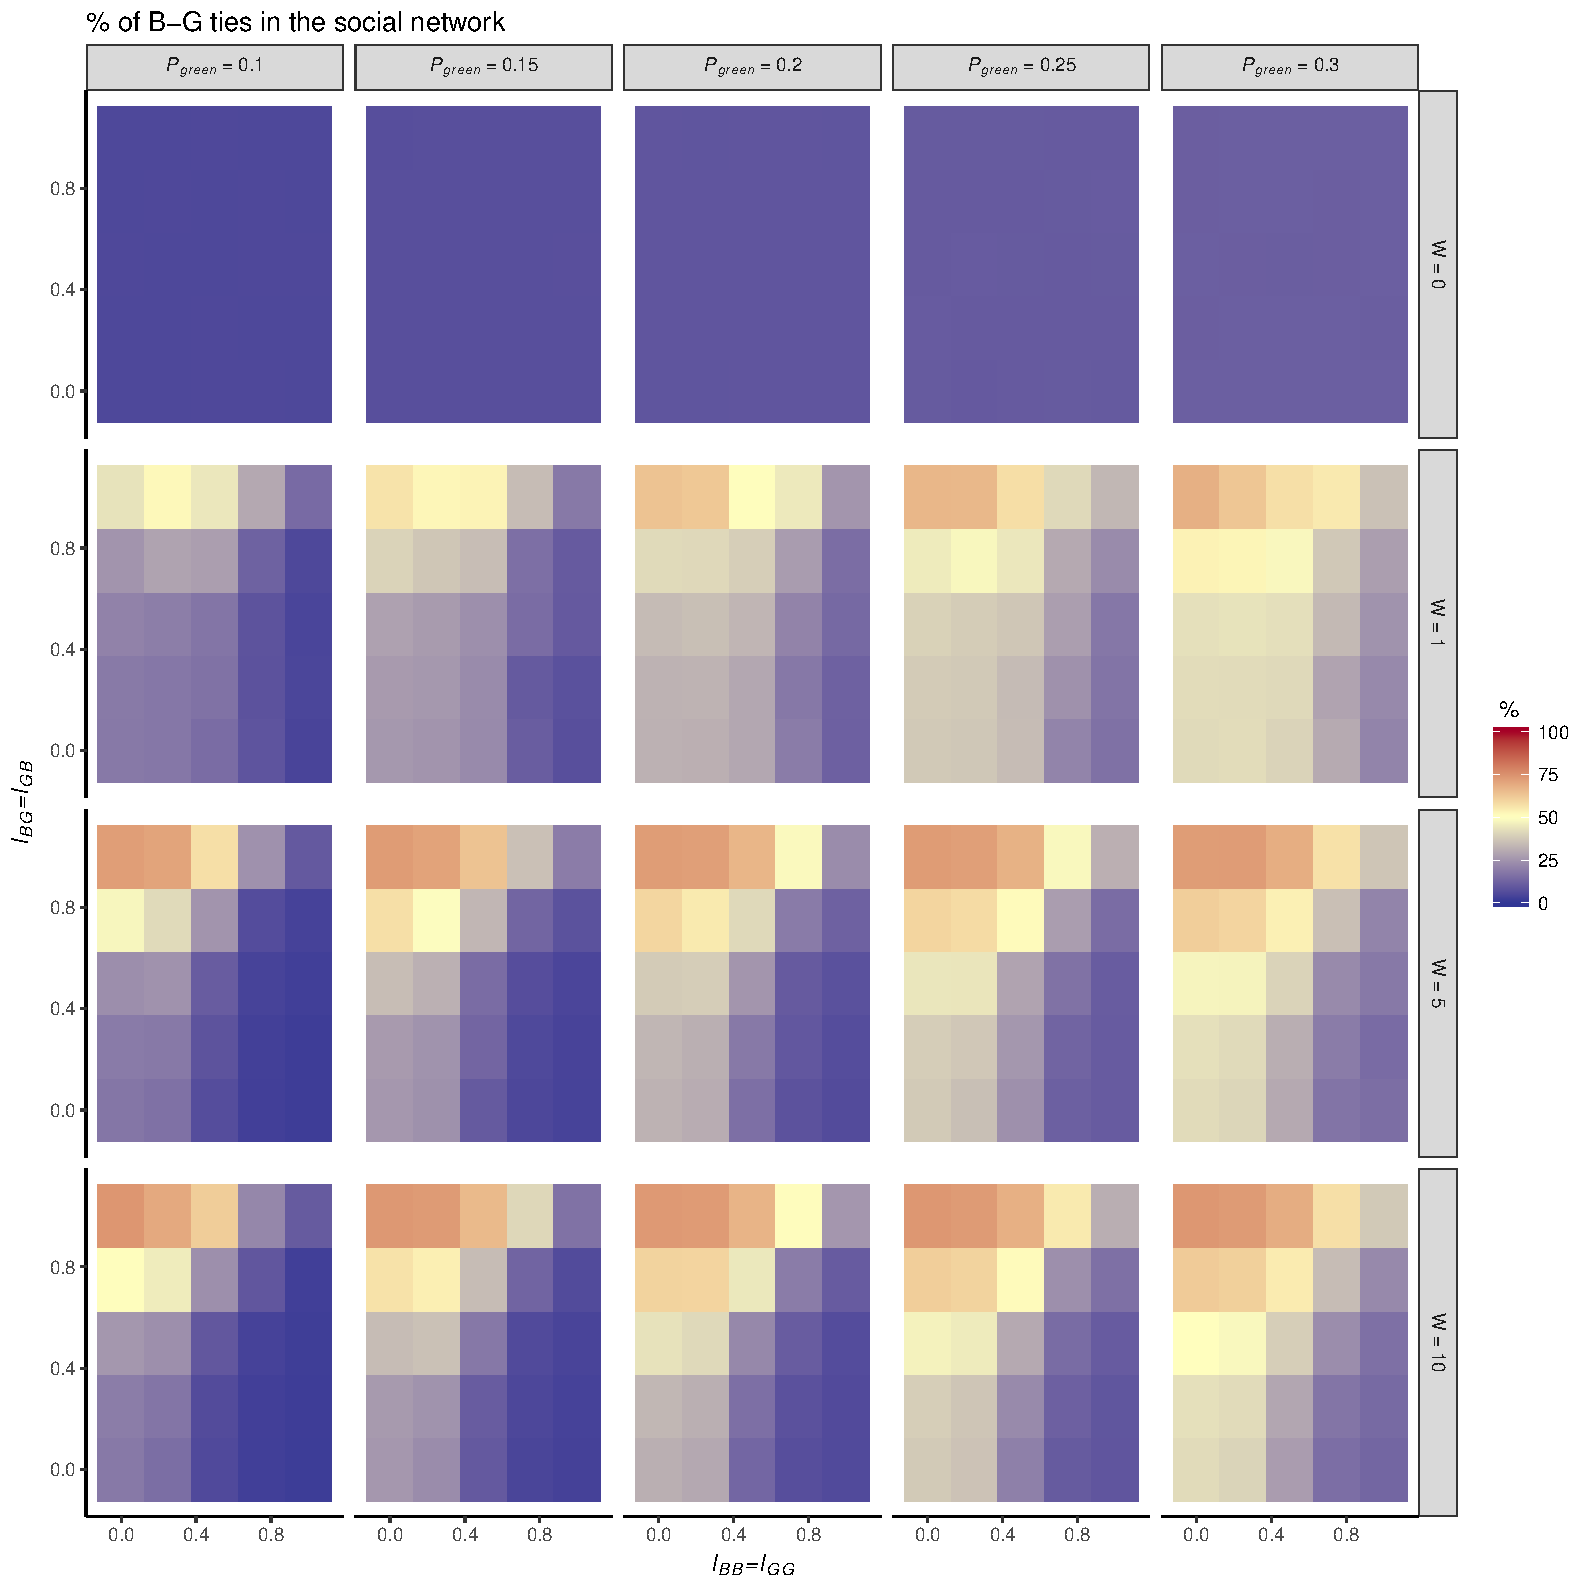
\includegraphics[trim={0cm 0cm 0.4cm 0cm}, clip, width=\linewidth]{figures/pctMixedTiesExperiment2.pdf}
	\end{minipage}
\end{figure}

Figure 10 shows that when the network is rigid ($ W = 0 $) the percentage of mixed ties in the network is low, regardless of the ``likenesses.'' This was expected, because if the network is static the ``likenesses'' towards in- and out-group influence strategy changes but not structural updates. For $ W > 0 $ the percentage of mixed ties is large for high values of the ``likeness'' towards the out-group and increases with both the relative size of the minority group and the frequency of structural updates. 

\subsection{Experiment 3}
The purpose of this experiment was to study the effect of the combined variations of likeness towards in-group, likeness towards out-group, size of minority group $ \mathcal{G}_{\mathcal{S}} $ and $ \gamma $ (game barrier), keeping the initial average connectivity $ n_{W} $, and  $ W $ constant. This experiment was important to confirm that increasing the cooperation barrier (game strength) would lead to cooperation to be wiped out, and determine whether or not the relative size of the minority group could significantly influence the value of $ \gamma $ for which full defection will result.

The initial average node degree was set at the constant value $ n_W = 16 $. The sweeping variables were the size of the minority group and the ``likenesses,'' which were set as in experiment 1, and the game barrier parameter, which was set $ \gamma = \{1,5,10,20\} $. 
\begin{figure}[ht!]
	\label{fig:strategyHostExperiment3}
	%\centering
	\begin{minipage}[c]{0.2\linewidth}
		\caption{Facets plot of the dominant strategy within the ``blue'' (majority) population after 500 cycles, obtained in experiment 3.}
	\end{minipage}
	\begin{minipage}[c]{0.75\linewidth}
		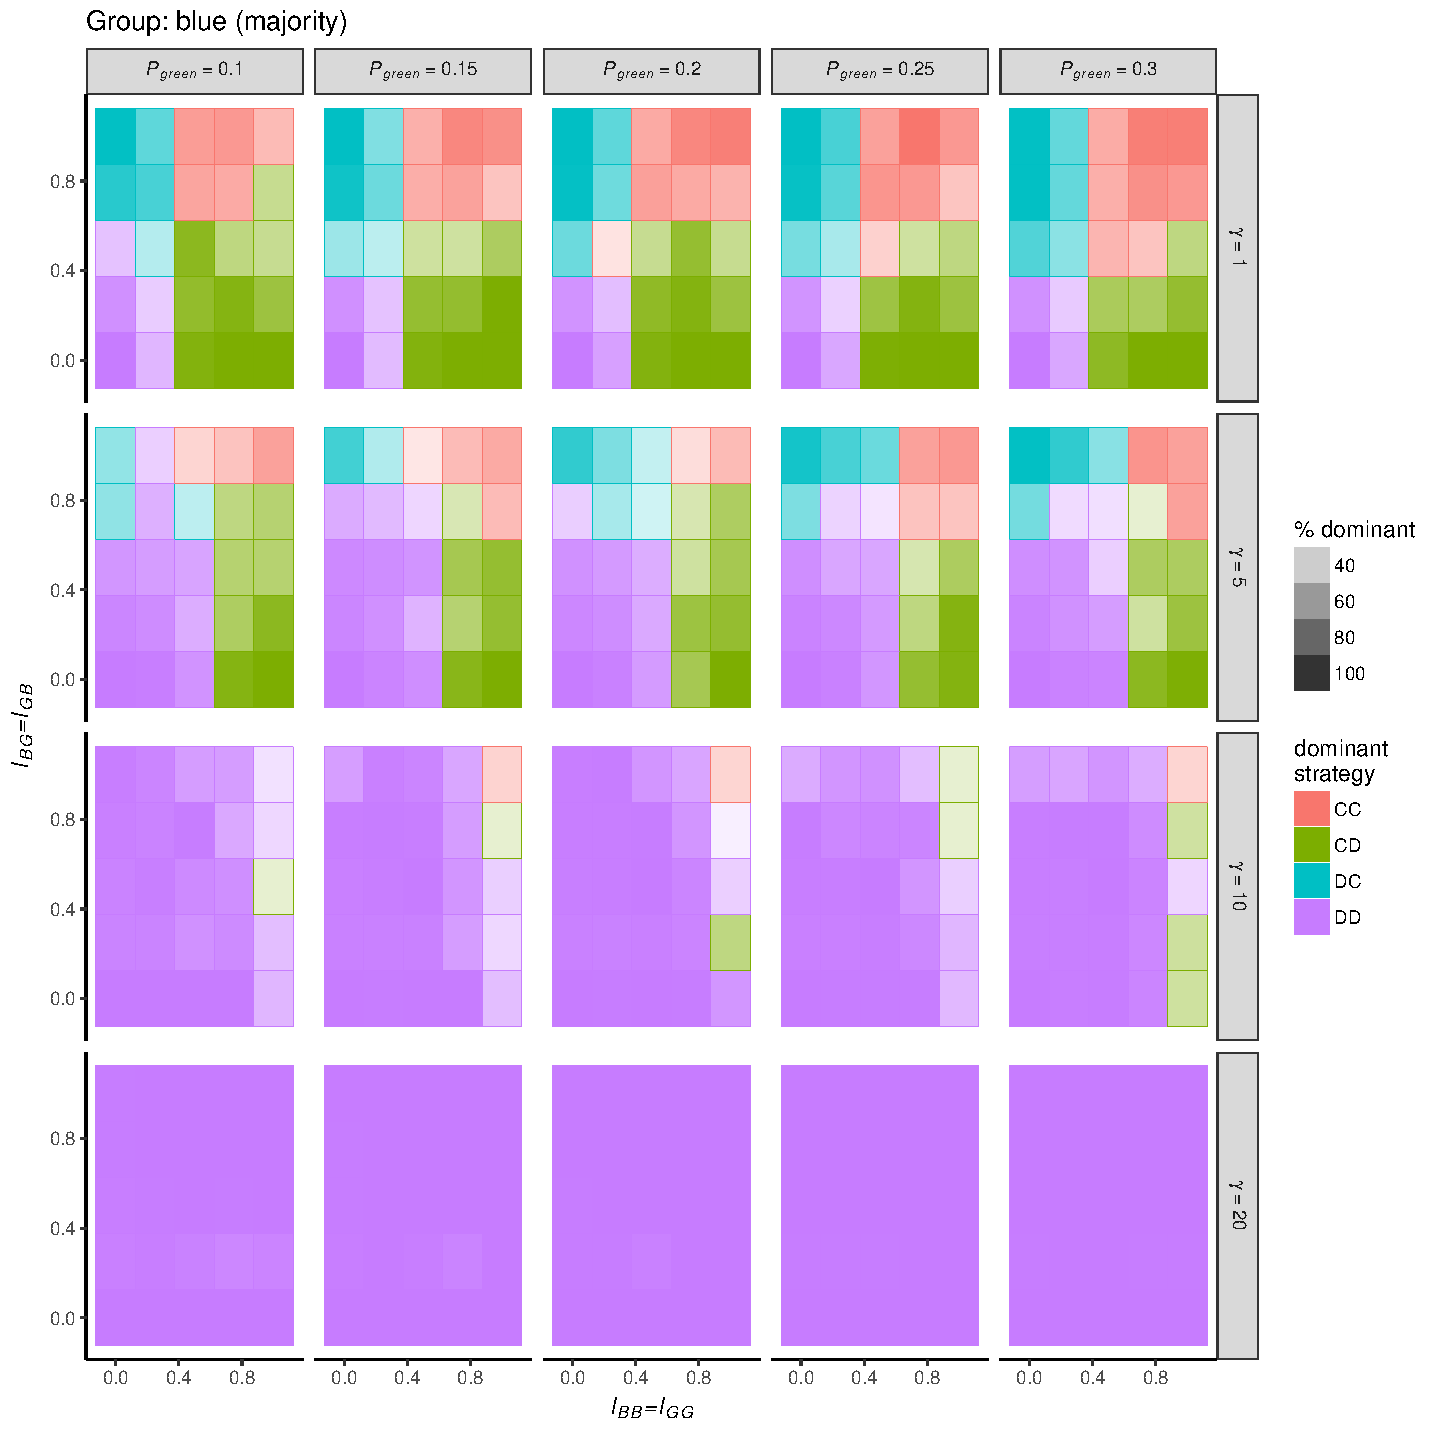
\includegraphics[trim={0cm 0cm 0.4cm 0cm}, clip, width=\linewidth]{figures/strategyHostExperiment3.pdf}
	\end{minipage}
\end{figure}

Figure 11 shows the facets plots of the dominant strategy for the ``blue'' (majority) population. This shows that in our model $ \gamma $ has indeed a strong impact on the dominant strategies, with an effect that is contrary to that of $ W $.

For low values of the game barrier (or strength)  any of the four possible strategies can emerge as dominant, depending on the group-tag barrier (``likeness''). For $ \gamma = 1 $ and 5, the effect of the relative size of the minority group on the emergence of ethnocentric or full cooperation is small. In contrast, increasing the value of $ \gamma $ from 1 to 5 leads to full defection, unless at least one of the ``likenesses'' is sufficiently high.

For $ \gamma = 10 $ ethnocentrism and full cooperation are only possible for very high values of ``likeness'' towards the in-group and large relative group size of the minority. The shading of tiles to the rightmost columns of the tiles for $ \gamma = 10 $ shows that on average cooperation does not extend to more than 40\% of the population (the results for the minority group are similar to those in figure 11). For $ \gamma = 20 $ cooperation is wiped out completely.

Figure 12 shows the percentage of mixed ties in the social network after 500 cycles. For $ \gamma = 1 $ and 5, the results are similar to those obtained in experiment 2 and shown in figure 10 for the cases of $ W > 0 $, with the difference that increasing $ \gamma $ has the same effect as decreasing $ W $. For $ \gamma = 10 $ and 20, the percentage of mixed ties increases with the relative size of the minority group. This result can be interpreted as follows. For large values of $ \gamma $ full defection dominates, but since agents are allowed to adjust their ties ($ W > 0 $) they continually search for (nonexistent or rare) cooperators.\footnote{This qualitative behavior is somewhat analogous to that in Schelling's segregation model when both the spatial agent density and the ``\%-similar-wanted'' are high, and agents just cannot find a spot where they are ``happy'' with their neighbors.} In these conditions, the influence of the group-tag barriers is no longer dominant (bottom row of tiles in figure 11) and the agents become indifferent to the group where they try to find cooperators. The larger relative size of the minority group then increases the probability of formation of mixed ties.
\begin{figure}[ht!]
	\label{fig:pctMixedTiesExperiment3}
	%\centering
	\begin{minipage}[c]{0.2\linewidth}
		\caption{Facets plot of the percentage of mixed ties (links between agents of different groups) after 500 cycles, obtained in experiment 3.}
	\end{minipage}
	\begin{minipage}[c]{0.75\linewidth}
		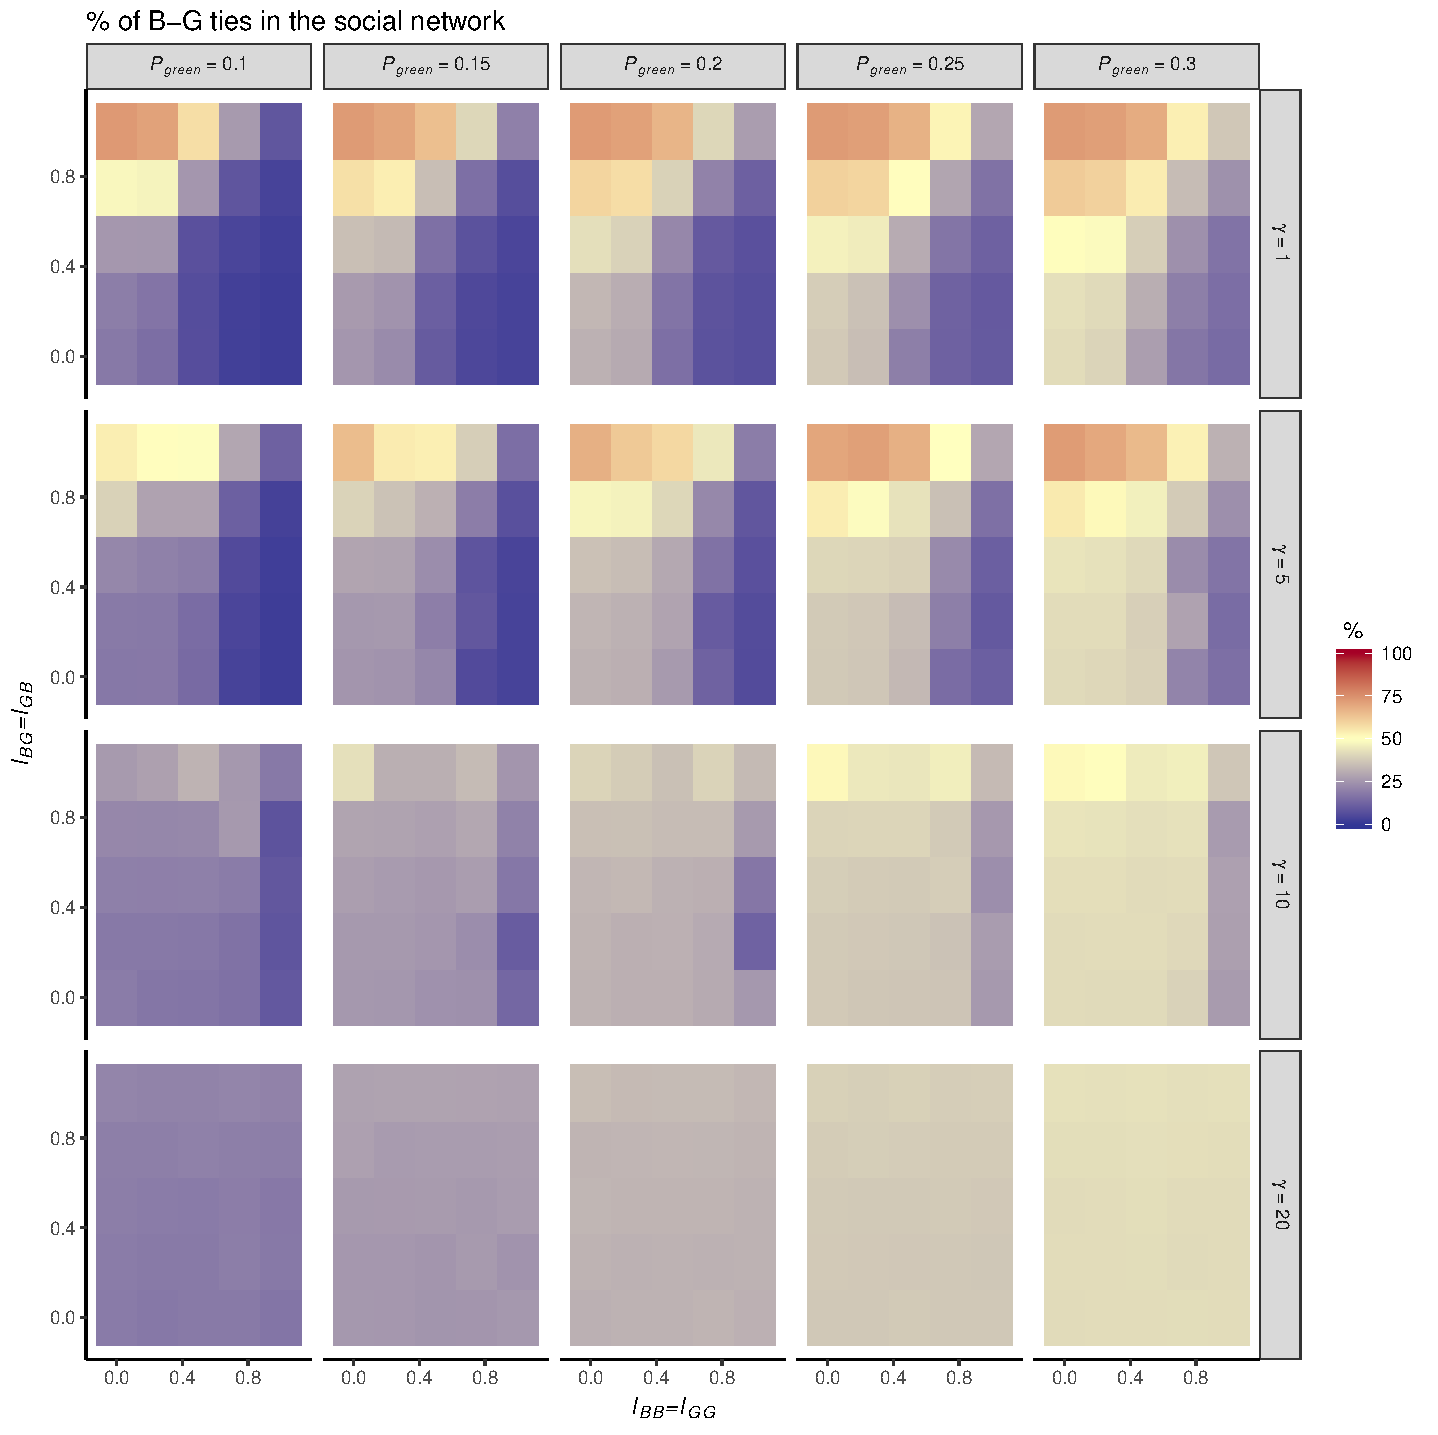
\includegraphics[trim={0cm 0cm 0.4cm 0cm}, clip, width=\linewidth]{figures/pctMixedTiesExperiment3.pdf}
	\end{minipage}
\end{figure}


\subsection{Experiment 4}
The purpose of this experiment was similar to that of Experiment 1, but for a non-symmetric likeness matrix, to determine whether or not different different dominant strategies would emerge in the majority and minority groups. The initial average connectivity $ n_W $ and the relative size of the minority group $ P_{green} $ were set as sweeping variables, with the values shown in table \ref{tab:Experiment1} for experiment 1. The other sweeping variables were $ l_{BG} = \{0,0.2,0.4,0.6,0.8\} $ and $ l_{GB} = \{0,0.2,0.4,0.6,0.8\} $.\footnote{The values of $ l_{BG} $ and $ l_{GB} $ used in this experiment are slightly different to those in the table \ref{tab:Experiment1}, so that a small bias towards in-group will remain.}
\begin{figure}[t!]
	\label{fig:strategyHostExperiment4}
	%\centering
	\begin{minipage}[c]{0.2\linewidth}
		\caption{Facets plot of the dominant strategy within the ``blue'' (majority) population after 500 cycles, obtained in experiment 4.}
	\end{minipage}
	\begin{minipage}[c]{0.75\linewidth}
		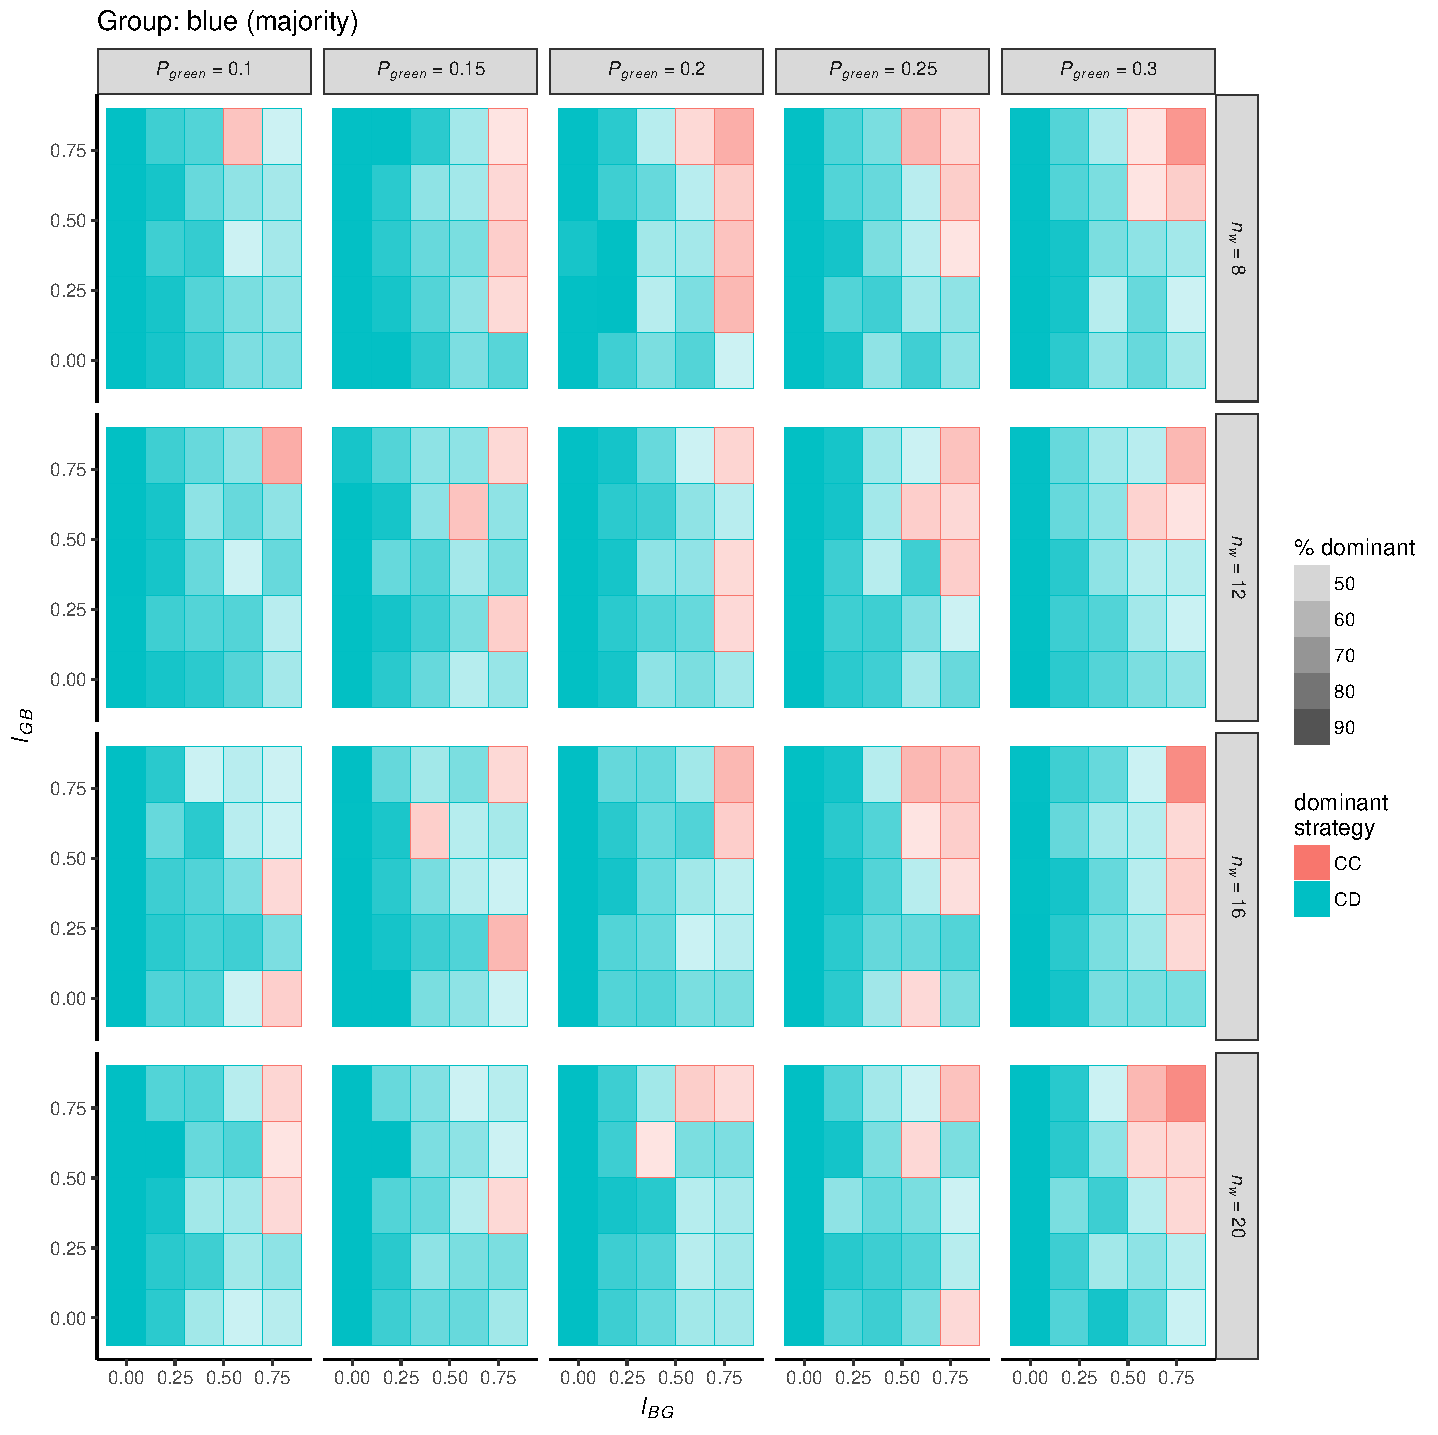
\includegraphics[trim={0cm 0cm 0.4cm 0cm}, clip, width=\linewidth]{figures/strategyHostExperiment4.pdf}
	\end{minipage}
\end{figure}

Figures 13 and 14 show the facets plots of the dominant strategy for the ``blue'' (majority) and ``green'' (minority) populations, respectively. These plots show that for the conditions of this experiment (particularly the fixed values of $ \gamma $ and $ W $ adopted) the dominant outcome is ethnocentrism, with full cooperation setting in for larger values of the ``likenesses'' towards the out-group, as expected. However, it can also be observed that except for a few cases the dominant strategy at the end of the simulations (averaged over all runs) turned out to be identical for both groups. The outcomes are also noisy, in the sense that the patterns of the transition from ethnocentrism to full cooperation are not clear. These shortcomings call for further study and refinement of the model. 
\begin{figure}[t!]
	\label{fig:strategyImmigrantExperiment4}
	%\centering
	\begin{minipage}[c]{0.2\linewidth}
		\caption{Facets plot of the dominant strategy within the ``green'' (minority) population after 500 cycles, obtained in experiment 4.}
	\end{minipage}
	\begin{minipage}[c]{0.75\linewidth}
		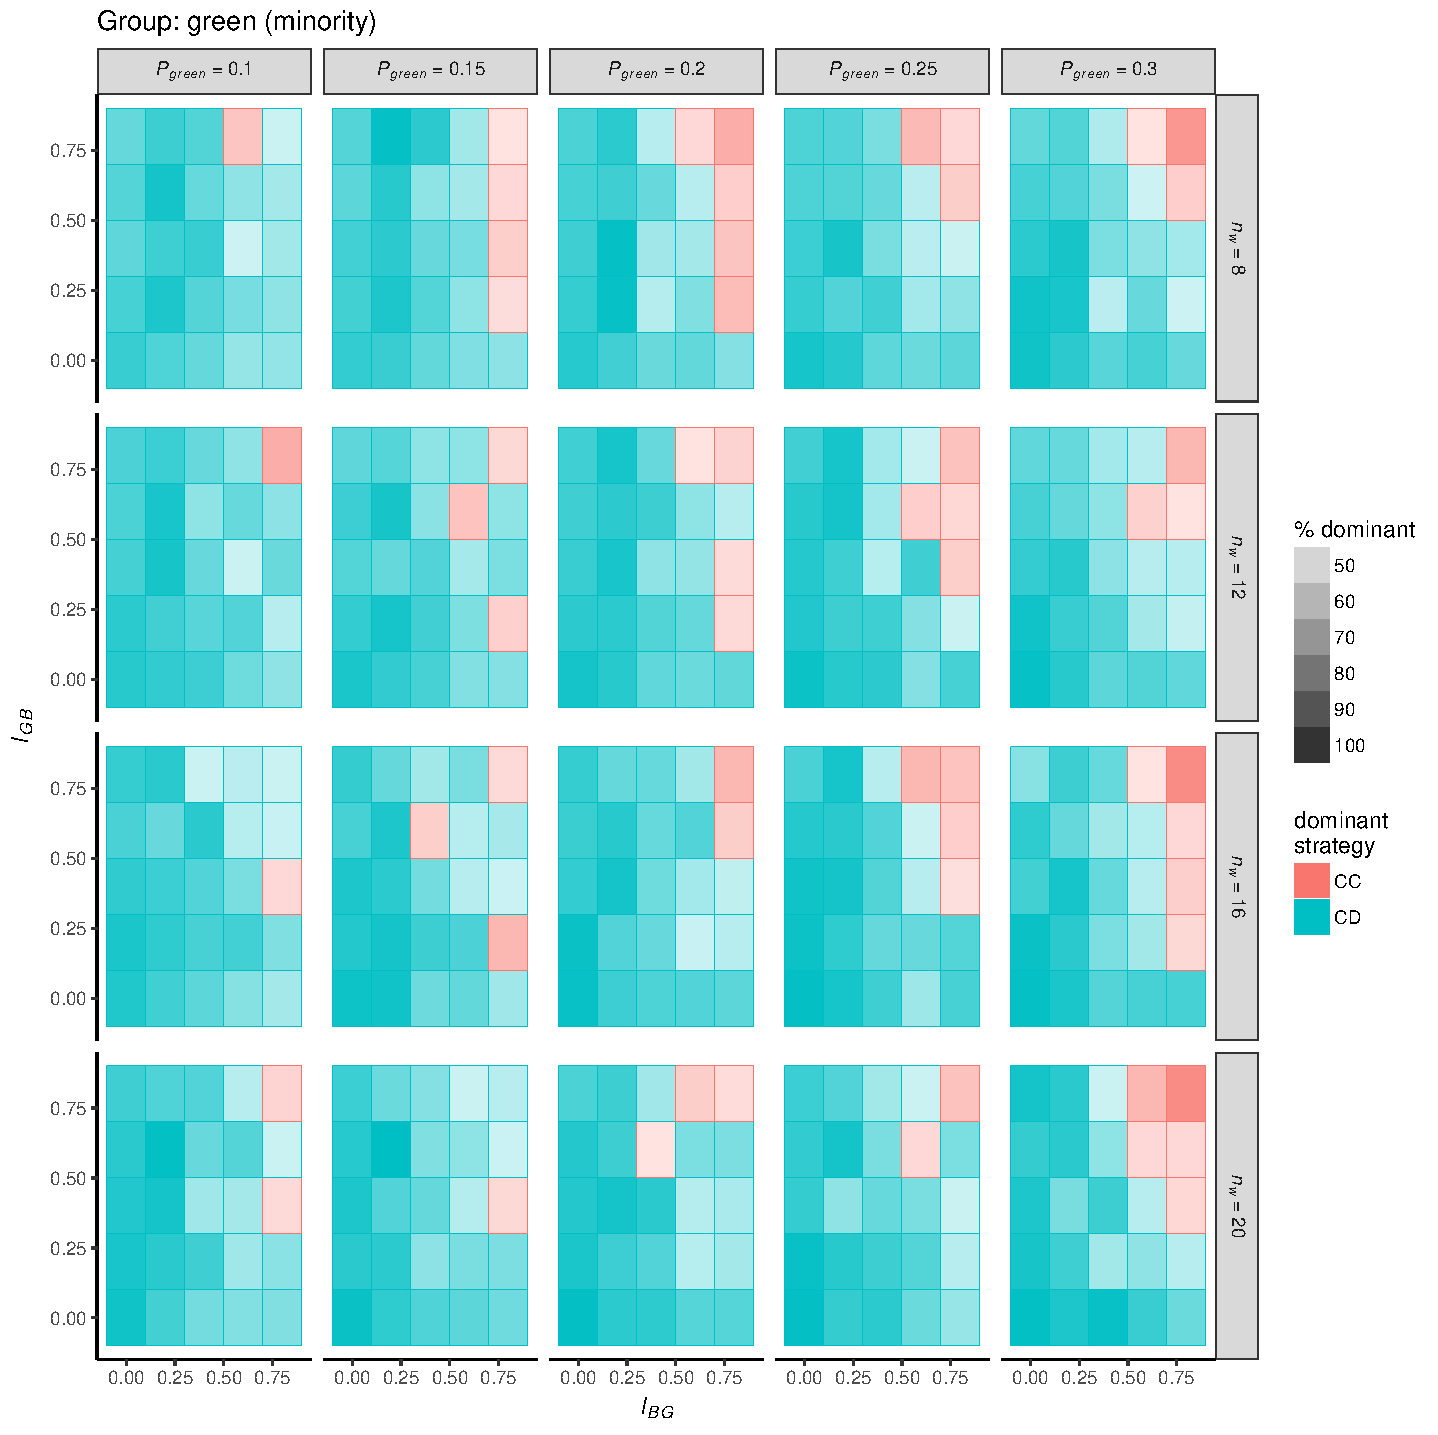
\includegraphics[trim={0cm 0cm 0.4cm 0cm}, clip, width=\linewidth]{figures/strategyImmigrantExperiment4.pdf}
	\end{minipage}
\end{figure}

\section{Discussion}
The experiments showed that the group-tag barrier (``likeness'' $ L $), frequency of structural adaptation $ W $ and game strength $ W $ are the variables with stronger impact on the resulting dominant strategies in our model. The relative size of the minority group and initial degree of connectivity do not affect the emergent strategies, but influence the resulting \% of mixed ties in the network. These general findings are consistent with previous results by Blau (1977) and Santos et al. (2006).

The results of experiment 1 showed that according to our model, the group-tag barriers can tip the dominant strategy towards any of the four possible outcomes, but diversity of strategies tends to persist. Both these features can be considered realistic. The relative size of the minority group and the initial degree of connectivity influence the \% of mixed ties at the end of the simulations. For high values of ``likeness'' towards the out-group, the minority can actually ended up with larger average node degree than the majority group. The difference between the average connectivity within majority and minority groups is also representative of real societies, but it may also be associated with limitations of the model, as discussed below.

The results of experiments 2 and 3 showed that $ \gamma $ and $ W $ have a strong impact on the emergence of cooperation, with opposite effects -- the former hinders cooperation, whereas the latter induces it. These results are consistent with the general theory of the PD game (e.g. Dixit et al. (2015)) and the models of games in networks (Santos et al. 2006). When the network is not allowed to adapt, cooperation is strongly hindered and the \% of mixed ties is totally dependent on initialization.

In experiments 1-3, the model yielded the same dominant strategies for both minority and majority groups. This was expected, since the ``likenesses'' towards in- and out-group were set equal for both majority and minority groups. In experiment 4, non-symmetric ``likeness'' matrices were imposed in a situation where either ethnocentric or full cooperation was expected. Although in some cases the dominant strategies of the two groups were different, there is a very strong tendency for the model to yield the same dominant structure for both majority and minority groups. This shows that after multiple iterations the mechanism of imitation on which the strategy update is based leads to the ``likeness'' barrier to becoming ineffective. Therefore, according to this model, simple imitation does not lead to diversity of cooperative behavior.



\section{Model Limitations}
Our model has some limitations, which are inherent to the variables and constructs used, and to limited representation of the mechanisms of cooperation and structural adaptation.

Considering first the issue of variables' and constructs, the intra- and inter-group relations were modeled using a single network and ``communality'' was taken as an abstract representation of feeling for group support. Although the latter is indeed a basic human need, social ties can be of multiple types (family, friends, acquaintances, workmates, etc.), each of which entails different levels of ``communality'' that are not easy to relate. Although our model cannot represent the joint effect of these influences, it is possible to simulate networks corresponding to different ``arenas'' (e.g. close friends or acquaintances) by setting the ``likeness'' and game barrier so that more intimate relationships would be more difficult to form. The formation of family ties, such as marriages and offspring, would require a much more complex model.

Although the mechanisms represented in the model are key, and their combination with group tag barriers provided plausible outcomes for the in- and out-group strategies and the networks of intra-group relationships, other important mechanisms were not modeled. First, memory of past interactions and implementation of simple strategies such as Tit-for-tat, Generous Tit-for-tat, or Grimm (Axelrod 1984; Nowak 2006a), in combination with the model of probabilistic imitation and structural change would provide a better representation of reciprocity. 

Another limitation of the model is reseting the communality at each cycle. This limitation is common to many existing models, including the Hammond/Axelrod and Jansson models of ethnocentrism (Hammond and Axelrod 2006; Jansson 2015) and the SPL model of cooperation in dynamic networks (Santos et al. 2006) and arises from the need to keep the communality stable at the individual and global level throughout the simulations. This limitation can only be overcome by considering the cost of maintaining social ties, but modeling this jointly with the strategy and structure updates while keeping the model parsimonious is indeed a challenging topic.

The constraint of keeping the network connected (as in Santos et al. (2006)) is also a limitation. This is necessary to avoid dissolution of the network into isolated nodes, particularly for low ``likenesses'' and strong cooperation barriers. This constraint is not unrealistic, for in real societies individuals are generally not completely isolated. This limitation is related to the one mentioned in the previous paragraph. Rewiring to neighbors of neighbors is also a potential limitation, but other alternatives would be equally open to criticism.

Two further limitations of the model are the use of fixed ``likeness'' barriers and the absence of population dynamics (such as offspring and immigration). Inclusion of these processes while preserving the simplicity of the model is also a challenging topic. 

\section{Conclusions}
In this work we presented a network ABM of ``abstract'' type for describing the co-evolution of ethnocentrism and social ties between two groups (majority and minority). In this model, agents have a group tag (``blue'' or ``green'') and a pair of strategies for cooperating or defecting when interacting with agents of identical or different tags (in- and out-group, respectively), as well as an attribute called ``communality'' that represents feeling of ``group solidarity'' and is modeled as the payoff of a social dilemma game. Interactions between pairs of agents are successful or unsuccessful depending on their relative ``likeness.'' If an interaction is successful, agents change their communality by playing a one-shot Prisoners' Dilemma (PD) game, and try to improve their communality by revising their strategy of by modifying their social ties.

The results of the computer experiments showed that the model can produce outcomes with each of the four possible strategies (full defection, cooperation towards out-group, cooperation towards in-group or ethnocentrism, and full cooperation) emerging as dominant. We now summarize how the results contribute to answer our research questions. 

Regarding the first research question, the group-tag barriers defined via the ``likeness'' matrix $ L $ play a key role in determining which strategy will emerge as dominant. The results also show that the model generates diversity, since strategies other than dominant persist within the majority and minority groups. Apart from the group-tag barrier, the two other parameters which have a strong impact on the outcomes are the frequency of structural updates $ W $ and the game barrier (or strength) $ \gamma $, which have opposite effects. Increasing $ W $ promotes ethnocentric and full cooperation, whereas increasing $ \gamma $ wipes out cooperation within the social network, leading to full defection. One important feature of our model is that strategies other than the dominant persist within both the majority and minority groups. To the best of our knowledge, this outcome is not well described in previous studies.  

Exploring our second research question, we found that the frequency of structural updates also influences the formation of mixed ties within the social network. When the network is kept rigid ($ W = 0 $) the social network is entirely dependent on initialization and there is no possibility for a network of mixed ties to grow. One interesting result is that when the ``likenesses'' towards the out-group are sufficiently large, the average node degree (and hence the communality) of the minority group can be substantially higher than that of the majority group. This behavior was also not reported in previous studies.

Finally, in answer to our third research question, we found that according to our model the relative size of the minority group and the initial network connectivity have a weaker impact on the resulting dominant strategies than the variables mentioned before, but influence the percentage of the network of mixed ties connecting agents belonging to different groups. 

In most simulations, the model yielded the same dominant strategies for both minority and majority groups, even when the tag-induced barriers were specified to be non-symmetric. This tendency for a common dominant strategy to emerge may be due to limited representation of the mechanisms of cooperation in the model.

The model described herein is part of work in progress and can be improved in many ways by incorporating more complete and realistic mechanisms. One of these is the influence of memory and learning effects in the evolution of individual strategies, instead of simple imitation. Another possible improvement is the representation of the group-tag barriers as a multiple-feature variable that can change in the course of interactions. Still another possible improvement is the formulation of a model of structural adaptation with a variable number of ties including both the reinforcement due to past successful interactions and the cost of keeping social ties.  

\begin{acknowledgements}
We are very grateful to Professor Francisco C. Santos at Instituto Superior T\'{e}cnico, Lisbon, Portugal, for his help and advice on implementing the submodel of network strategy and structural updates. We also thank Senior Engineer Sigurd Kristian Brinch of the Department of Information and Communication Technologies at the University of Agder for his help with providing access to computer resources that were essential for the completion of the present work.
\end{acknowledgements}

% BibTeX users please use one of
%\bibliographystyle{spbasic}      % basic style, author-year citations
%%%%\bibliographystyle{spmpsci}      % mathematics and physical sciences
%\bibliographystyle{plain}
%\bibliographystyle{spphys}       % APS-like style for physics
%%%%\bibliography{Ethnocentrism}   % name your BibTeX data base

% Non-BibTeX users please use
%\begin{thebibliography}{}
%
% and use \bibitem to create references. Consult the Instructions
% for authors for reference list style.
%
%\bibitem{RefJ}
% Format for Journal Reference
%Author, Article title, Journal, Volume, page numbers (year)
% Format for books
%\bibitem{RefB}
%Author, Book title, page numbers. Publisher, place (year)
% etc
%\end{thebibliography}
\begin{thebibliography}{10}
	\providecommand{\url}[1]{{#1}}
	\providecommand{\urlprefix}{URL }
	\expandafter\ifx\csname urlstyle\endcsname\relax
	\providecommand{\doi}[1]{DOI~\discretionary{}{}{}#1}\else
	\providecommand{\doi}{DOI~\discretionary{}{}{}\begingroup
		\urlstyle{rm}\Url}\fi
	
	\bibitem{Ahmed2007}
	Ahmed, A.M.: Group identity, social distance and intergroup bias.
	\newblock Journal of Economic Psychology \textbf{28}(3), 324--337 (2007)
	
	\bibitem{Allport1958}
	Allport, G.W.: {The nature of prejudice}.
	\newblock {Doubleday Anchor} (1958)
	
	\bibitem{Axelrod1997}
	Axelrod, R.: {The Dissemination of Culture: A Model with Local Convergence and
		Global Polarization}.
	\newblock {Journal of Conflict Resolution} \textbf{41}, 203--226 (1997)
	
	\bibitem{Blalock1967}
	Blalock, H.M.: {Toward a theory of minority-group relations}.
	\newblock {Wiley} (1967)
	
	\bibitem{Blau1977}
	Blau, P.M.: {A Macrosociological Theory of Social Structure}.
	\newblock {American Journal of Sociology} \textbf{83}(1), 26--54 (1977)
	
	\bibitem{Blumer1958}
	Blumer, H.: {Race prejudice as a sense of group position}.
	\newblock {The pacific Sociological Review} \textbf{1}, 3--7 (1958)
	
	\bibitem{Brewer1979}
	Brewer, M.B.: The role of ethnocentrism in intergroup conflict.
	\newblock In: W.G. Austin, S.~Worchel (eds.) The psychology of intergroup
	relations, pp. 88--102. Brooks/Cole, Monterey, CA (1979)
	
	\bibitem{Brewer1999}
	Brewer, M.B.: The psychology of prejudice: Ingroup love or outgroup hate?
	\newblock Journal of Social Issues \textbf{55}(3), 429--444 (1999)
	
	\bibitem{Chirot2001}
	Chirot, D., Seligman, M.E.P.: Ethno political warfare: Causes, consequences,
	and possible solutions.
	\newblock American Psychological Association, Washington, D.C. (2001)
	
	\bibitem{Dennen1995}
	van~der Dennen, J.M.G.: The origin of war.
	\newblock Origin Press, Groningen, Netherlands (1995)
	
	\bibitem{ADSSDR2015}
	Dixit, A., Skeath, S., Reiley, D.: {Games of Strategy}, 4th edn.
	\newblock {W. W. Norton \& Company}, {New York and London} (2015)
	
	\bibitem{Doise1972}
	Doise, W., Csepeli, G., Dann, H.D., Gouge, C., larsen, K., Ostell, A.: An
	experimental investigation into the formation of intergroup representations.
	\newblock {European Journal of Social Psychology} \textbf{2}, 202--204 (1972)
	
	\bibitem{Ebel2002}
	Ebel, H., Bornholdt, S.: Coevolutionary games on networks.
	\newblock Physical Review E \textbf{66}(056118), 1--8 (2002)
	
	\bibitem{Epstein2006}
	Epstein, J.M.: {Generative Social Science. Studies in Agent-Based Computational
		Modeling}.
	\newblock {Princeton University Press}, Princeton, New Jersey (2006)
	
	\bibitem{NigelGilbert2007a}
	Gilbert, N.: {Agent-Based Models (Quantitative Applications in Social
		Sciences)}.
	\newblock {Sage Publications}, Los Angeles and London and New Dehli and
	Singapore (2007)
	
	\bibitem{Hammond2006}
	Hammond, R.A., Axelrod, R.: {The Evolution and Ethnocentrism}.
	\newblock {Journal of Conflict Resolution} \textbf{50}(6), 1--11 (2006)
	
	\bibitem{Jackson2008}
	Jackson, M.O.: {Social and Economic Networks}.
	\newblock {Princeton University Press} (2008)
	
	\bibitem{Jansson2015}
	Jansson, F.: {What games support the evolution of an ingroup bias?}
	\newblock Journal of Theoretical Biology \textbf{373}, 100--110 (2015)
	
	\bibitem{Kinder1998}
	Kinder, D.R.: Opinion and action in the realm of politics.
	\newblock In: D.T. Gilbert, S.T. Fiske, G.~Lindzey (eds.) Handbook of social
	psychology, pp. 778--867. McGraw-Hill, New York, NY (1998)
	
	\bibitem{Kramer1984}
	Kramer, R.M., Brewer, M.B.: Effects of group identity on resource use in a
	simulated commons dilemma.
	\newblock Journal of Personality and Social Psychology \textbf{46}(5),
	1044--1057 (1984)
	
	\bibitem{LeVine1972}
	LeVine, R.A., Campbell, D.T.: Ethnocentrism: Theories of conflict, ethnic
	attitudes and group behavior.
	\newblock John Wiley \& Sons, Oxford, England (1972)
	
	\bibitem{Macy2002}
	Macy, M.W., Flache, A.: Learning dynamics in social dilemmas.
	\newblock Proceedings of the National Academy of Sciences of the United States
	of America \textbf{99}(3), 7229--7236 (2002)
	
	\bibitem{McPherson2001}
	McPherson, M., Smith-Lovin, L., Cook, J.M.: {Birds of a Feather: Homophily in
		Social Networks}.
	\newblock {Annual Review of Sociology} \textbf{27}, 415--444 (2001)
	
	\bibitem{Nowak2006a}
	Nowak, M.A.: {Evolutionary Dynamics. Exploring the Equations of Life}.
	\newblock Belknap Press (2006)
	
	\bibitem{Nowak2006}
	Nowak, M.A.: {Five rules for the evolution of cooperation}.
	\newblock Science \textbf{314}(5805), 1560--1563 (2006a)
	
	\bibitem{Ohtsuki2006}
	Ohtsuki, H., Hauert, C., Lieberman, E., Nowak, M.A.: {A simple rule for
		evolution of cooperation on graphs and social networks}.
	\newblock Nature \textbf{441}, 502--505 (2006)
	
	\bibitem{Perreault1999}
	Perreault, S., Bourhis, R.Y.: Ethnocentrism, social identification, and
	discrimination.
	\newblock Personality and Social Psychology Bulletin \textbf{25}(1), 92--103
	(1999)
	
	\bibitem{Pinheiro2016}
	Pinheiro, F., Santos, F.C., Pacheco, J.M.: {Linking Individual and Collective
		Behavior in Adaptive Social Networks}.
	\newblock {Physical Review Letters} p. 128702 (2016)
	
	\bibitem{Pinheiro2012}
	Pinheiro, F.L., Pacheco, J.M., Santos, F.C.: {From Local to Global Dilemmas in
		Social Networks}.
	\newblock PLoS ONE \textbf{7}(2), 1--6 (2012)
	
	\bibitem{RCT2016}
	{R Core Team}: R: A Language and Environment for Statistical Computing.
	\newblock R Foundation for Statistical Computing, Vienna, Austria, version
	3.2.5 edn. (2016)
	
	\bibitem{AnatolRapoport1999}
	Rapoport, A.: {Two-Person Game Theory}.
	\newblock {Dover Publications}, {Mineola, New York} (1999)
	
	\bibitem{Axelrod1984}
	{Robert Axelrod}: The Evolution of Co-operation.
	\newblock {Basic Books, Inc.}, New York (1984)
	
	\bibitem{Santos2006}
	Santos, F.C., Pacheco, J.M., Lenaerts, T.: Cooperation prevails when
	individuals adjust their social ties.
	\newblock {PLoS Computational Biology} \textbf{2}(10), 1284--1291 (2006)
	
	\bibitem{Santos2006a}
	Santos, F.C., Pacheco, J.M., Lenaerts, T.: {Evolutionary dynamics of social
		dilemmas in structured heterogeneous populations}.
	\newblock PNAS \textbf{103}(9), 3490--3494 (2006)
	
	\bibitem{Santos2016}
	Santos, F.P., Santos, F.C., Pacheco, J.M.: {Social Norms of Cooperation in
		Small-Scale Societies}.
	\newblock {PLoS Computational Biology} \textbf{12}(1), 1--13 (2016)
	
	\bibitem{Schelling1971}
	Schelling, T.C.: {Dynamic Models of Segregation}.
	\newblock {Journal of Mathematical Sociology} \textbf{1}, 143--186 (1971)
	
	\bibitem{Schelling2006}
	Schelling, T.C.: {Micromotives and Macrobehavior}, revised edn.
	\newblock {W. W. Norton \& Company} (2006)
	
	\bibitem{Skyrms2000}
	Skyrms, B., Pemantle, R.: A dynamic model of social network formation.
	\newblock Proceedings of the National Academy of Sciences of the United States
	of America \textbf{97}(16), 9340--9346 (2000)
	
	\bibitem{Smith1982}
	Smith, J.M.: Evolution and the Theory of Games.
	\newblock Cambridge University Press, Cambridge, United Kingdom (1982)
	
	\bibitem{Tajfel1971}
	Tajfel, H., Billig, M.G., Bundy, R.P., Flament, C.: Social categorization and
	intergroup behaviour.
	\newblock {European Journal of Social Psychology} \textbf{1}, 149--178 (1971)
	
	\bibitem{Thiele2014}
	Thiele, J.C.: {R} marries {NetLogo}: Introduction to the {RNetLogo} package.
	\newblock Journal of Statistical Software \textbf{58}(2), 1--41 (2014)
	
	\bibitem{Thiele2012}
	Thiele, J.C., Kurth, W., Grimm, V.: {RNetLogo}: An {R} package for running and
	exploring individual-based models implemented in {NetLogo}.
	\newblock Methods in Ecology and Evolution \textbf{3}(3), 480--483 (2012)
	
	\bibitem{Watts1998}
	Watts, D.J., Strogatz, S.H.: {Collective dynamics of `small-world' networks}.
	\newblock Nature \textbf{393}, 440--442 (1998)
	
	\bibitem{Wilensky:1999}
	Wilensky, U.: Netlogo.
	\newblock http://ccl.northwestern.edu/netlogo/, Center for Connected Learning
	and Computer-Based Modeling, Northwestern University, Evanston, IL (1999).
	\newblock \urlprefix\url{http://ccl.northwestern.edu/netlogo/}
	
	\bibitem{Yamagishi2009}
	Yamagishi, T., Mifune, N.: Social exchange and solidarity: in-group love or
	out-group hate?
	\newblock Evolution and Human Behavior \textbf{30}, 229--237 (2009)
	
\end{thebibliography}


\end{document}
% end of file template.tex

